\newcommand{\V}{\mathbb{V}}
\newcommand{\R}{\mathbb{R}}
\newcommand{\mm}{\mathcal{M}}
\newcommand{\dd}{\mathrm{d}}
\newcommand{\w}{\omega}
\newcommand{\wg}{\wedge}
\newcommand{\be}{\textbf{e}}
\newcommand{\red}[1]{\textcolor{red}{#1}}
\newcommand{\purple}[1]{\textcolor{purple}{#1}}
\newcommand{\g}{\Sigma_g}
\renewcommand{\S}{\mathbb{S}}
\renewcommand{\P}{\mathbb{R}\mathbb{P}}
\renewcommand{\gg}{\widetilde{\Sigma}_g}
\newcommand{\sen}{\operatorname{sen}}
\newcommand{\prr}{\text{pr}_2}
\newcommand{\pr}{\text{pr}_1}
\newcommand{\nn}{\mathcal{N}}

\newcommand{\parent}[1]{\left( #1 \right)}
\newcommand{\colch}[1]{\left\{ #1 \right\}}
\newcommand{\codim}{\operatorname{codim}}
\newcommand{\diam}{\operatorname{diam}}







































\iffalse

\newcommand{\be}{\mathbf{e}}
\newcommand{\T}{\mathscr{T}}
\newcommand{\V}{\mathbb{V}}
\newcommand{\mm}{\mathcal{M}}
\newcommand{\nn}{\mathcal{N}}
\newcommand{\parent}[1]{\left( #1 \right)}
\newcommand{\dx}{\mathrm{d}x}
\newcommand{\dr}{\mathrm{d}r}
\newcommand{\dd}{\mathrm{d}}
\newcommand{\Id}{\mathrm{Id}}
\newcommand{\suave}[1]{\mathscr{C}^{\infty}\parent{#1}}

\newcommand{\bee}{\widetilde{\be}}
\newcommand{\Rmm}[4]{\Rm\parent{#1,#2}#3, #4}
\newcommand{\segf}{\mathbf{\mathrm{\RNum{2}}}}
\newcommand{\RNum}[1]{\textbf{\uppercase\expandafter{\romannumeral #1\relax}}}
\newcommand{\conj}[2]{\{#1 \ \vert \ #2 \}}
\newcommand{\tioC}[2]{\widetilde{#1}^{#2}}
\newcommand{\tioB}[2]{\widetilde{#1}_{#2}}
\newcommand{\Munderbrace}[2]{\begingroup \color{violet} \underbrace{\color{black} #1 }_{\color{violet} #2 } \endgroup}
\newcommand{\Bunderbrace}[2]{\begingroup \color{gal} \underbrace{\color{black} #1 }_{\color{gal} #2 } \endgroup}
\newcommand{\Moverbrace}[2]{\begingroup \color{violet} \overbrace{\color{black} #1 }^{\color{violet} #2 } \endgroup}
\renewcommand{\l}{\ell}

\newcommand{\tr}{\operatorname{tr}}
\newcommand{\Ric}{\mathrm{Ric}}
\newcommand{\Rm}{\mathrm{Rm}}
\newcommand{\Lip}{\mathrm{Lip}}
\newcommand{\dist}{\mathrm{dist}}
\newcommand{\Scal}{\mathrm{Scal}}
\newcommand{\cn}{\nabla}
\newcommand{\KN}{\mathbin{\bigcirc\mspace{-15mu}\wedge\mspace{4mu}}}

\fi

\documentclass[a4paper, 12pt, twoside]{article}
\usepackage[utf8]{inputenc}
\usepackage[T1]{fontenc}
\usepackage[portuguese]{babel}
\usepackage[dvipsnames]{xcolor}
\usepackage{amsmath, amsfonts}
\usepackage{amsthm}
\usepackage{etoolbox}
\usepackage{lmodern}
\usepackage{lastpage}
\usepackage{totcount}
\everymath{\displaystyle}
%\usepackage[sc]{mathpazo}
%\linespread{1.05} 
\usepackage{mathrsfs}



\usepackage{hyperref}
\hypersetup{
    colorlinks=true, %set true if you want colored links
    linktoc=all,     %set to all if you want both sections and subsections linked
    linkcolor=black,
    citecolor = teal   %choose some color if you want links to stand out
}

\usepackage{cleveref}


\crefname{deff}{}{definitions}
\crefname{exem}{}{exemplos}
\crefname{col}{}{corolários}
\crefname{equation}{}{equações}
\creflabelformat{equation}{#2{\bf{\color{blue}(#1)}}#3}
\crefname{teorema}{}{teoremas}
\crefname{oobs}{observação}{observações}
\creflabelformat{oobs}{#2\bf{\color{violet}(O.#1)}#3}
\crefname{lema}{}{lemas}
\creflabelformat{lema}{#2\bf{\color{gal}(L.#1)}#3}
\crefname{proposicao}{}{proposições}
\creflabelformat{deff}{#2\bf{\color{cyan}(D.#1)}#3}
\creflabelformat{exem}{#2\bf{\color{BlueViolet}(E.#1)}#3}
\creflabelformat{col}{#2\bf{\color{Aquamarine}(C.#1)}#3}
\creflabelformat{proposicao}{#2{\bf\color{Sepia}(P.#1)}#3}



\makeatletter
\patchcmd{\f@nch@head}{\rlap}{\color{BlueViolet}\rlap}{}{}
%\patchcmd{\headrule}{\hrule}{\color{TealBlue}\hrule}{}{}
\patchcmd{\f@nch@foot}{\rlap}{\color{BlueViolet}\rlap}{}{}
\patchcmd{\footrule}{\hrule}{\color{green}\hrule}{}{}
\makeatother

\newtheorem{exerc}{Questão}
\usepackage{float,framed}
\setlength{\intextsep}{2pt}
\setlength{\textfloatsep}{2pt}
\newfloat{Box}{H}{0ob}
\newenvironment{Mybox}{\begin{Box}\begin{framed}\begin{exerc}}{\end{exerc}\end{framed}\end{Box}}



%\usepackage[shortlabels]{enumitem}

\usepackage[a4paper,bottom=0.9in,top=0.9in,left=0.3in,right=0.3in]{geometry}

\usepackage{mathtools}
\usepackage{fancyhdr}
\usepackage{lipsum}
\usepackage{enumerate}
\usepackage{rotating}
\usepackage{enumitem}

\usepackage{lastpage}
\usepackage{graphicx}
\everymath{\displaystyle}
\newcommand{\p}{\partial}
\pagestyle{fancy}
\renewcommand{\footrulewidth}{0.4pt}
\fancyhf{}
\rhead{\color{BlueViolet}\textbf{2023/1}}
%\chead{\textbf{\thepage}}
\lhead{\color{BlueViolet}\textbf{DINÂMICA DE EQUAÇÕES DE EVOLUÇÃO}}
\lfoot{\textbf{MATHEUS A. R. M. HORÁCIO}}
%\rfoot{\textbf{MATRÍCULA: 17/0110923 }}
\rfoot{\textbf{Página \thepage \ de \pageref*{LastPage}}}
  \renewcommand\headrule{%

 \color{BlueViolet}\noindent\makebox[\linewidth]{\rule{\paperwidth}{1pt}}
}
  \renewcommand\footrule{%

 \color{BlueViolet}\noindent\makebox[\linewidth]{\rule{\paperwidth}{1pt}}
}


\newcommand{\om}{\mathbb{M}}

\newcommand{\jps}[1]{\textcolor{blue}{#1}}
%\newcommand{\red}[1]{\textcolor{red}{#1}}
\newcommand{\pur}[1]{\textcolor{purple}{#1}}
\newcommand{\maggg}[1]{\textcolor{magenta}{#1}}

%\usepackage{color}
%\definecolor{SAEblue}{rgb}{0, .62, .91}
%\renewcommand\theequation{\red{{\arabic{equation}}}}


\makeatletter
\let\mytagform@=\tagform@
\def\tagform@#1{\maketag@@@{\bfseries\jps{(\ignorespaces#1\unskip\@@italiccorr)}}\hspace{3mm}}
\renewcommand{\eqref}[1]{\textup{\mytagform@{\ref{#1}}}}
\makeatother

\newcommand{\quotes}[1]{``#1''}

\definecolor{navybluegalaxy}{RGB}{0, 36, 93}
\definecolor{gal}{RGB}{0, 7, 111}
%\chead{\textbf{\thepage}}
\theoremstyle{definition}
\newtheorem{def*}{Definição}
\newtheorem{quest}{Questão}
\newtheorem{quest2}{Questão}
\newcommand{\ve}{\varepsilon}
\newcommand{\lnr}{\left\|}
\newcommand{\ssum}{\displaystyle\sum}
\newcommand{\rnr}{\right\|}
%\newcommand{\R}{\mathbb{R}}
\newcommand{\C}{\mathbb{C}}
\DeclareMathOperator{\hol}{Hol}
\newtheorem*{obs*}{Notação}
%\newtheorem*{oobs}{Observação}
\newtheorem{sublema}{Sub-lema}
\renewcommand{\qedsymbol}{\rule{0.7em}{0.7em}}
\newenvironment{demm}{\smallskip \noindent{\bf \underline{Demonstração:}}}
{\begin{flushright} $\qedsymbol$\end{flushright}\smallskip}
\newenvironment{dem}{\smallskip \noindent{\bf \underline{Solução:}}}
{\begin{flushright} $\qedsymbol$\end{flushright}\smallskip}

\newtheoremstyle{theoremOOBS}% name of the style to be used
  {\topsep}% measure of space to leave above the theorem. E.g.: 3pt
  {\topsep}% measure of space to leave below the theorem. E.g.: 3pt
  {}% name of font to use in the body of the theorem
  {1pt}% measure of space to indent
  {\bfseries\color{violet}}% name of head font
  {}% punctuation between head and body
  { }% space after theorem head; " " = normal interword space
  {\underline{\thmname{#1} (\thmnumber{O.#2})\textbf{\thmnote{ (#3)}.}}}

\theoremstyle{theoremOOBS}
\newtheorem{oobs}{Observação}

\newtheoremstyle{theoremEX}% name of the style to be used
  {\topsep}% measure of space to leave above the theorem. E.g.: 3pt
  {\topsep}% measure of space to leave below the theorem. E.g.: 3pt
  {}% name of font to use in the body of the theorem
  {1pt}% measure of space to indent
  {\bfseries\color{BlueViolet}}% name of head font
  {}% punctuation between head and body
  { }% space after theorem head; " " = normal interword space
  {\underline{\thmname{#1} (\thmnumber{E.#2})\textbf{\thmnote{ (#3)}.}}}

\theoremstyle{theoremEX}
\newtheorem{exem}{Exemplo}


\newtheoremstyle{theoremLEM}% name of the style to be used
  {\topsep}% measure of space to leave above the theorem. E.g.: 3pt
  {\topsep}% measure of space to leave below the theorem. E.g.: 3pt
  {}% name of font to use in the body of the theorem
  {1pt}% measure of space to indent
  {\bfseries\color{navybluegalaxy}}% name of head font
  {}% punctuation between head and body
  { }% space after theorem head; " " = normal interword space
  {\underline{\thmname{#1} (\thmnumber{L.#2})\textbf{\thmnote{ (#3)}.}}}

\theoremstyle{theoremLEM}
\newtheorem{lema}{Lema}

\newtheoremstyle{theoremTEO}% name of the style to be used
  {\topsep}% measure of space to leave above the theorem. E.g.: 3pt
  {\topsep}% measure of space to leave below the theorem. E.g.: 3pt
  {\itshape}% name of font to use in the body of the theorem
  {5pt}% measure of space to indent
  {\bfseries\color{gal}}% name of head font
  {}% punctuation between head and body
  { }% space after theorem head; " " = normal interword space
  {\underline{\thmname{#1} (\thmnumber{T.#2})\textbf{\thmnote{ (#3)}.}}}
  


\theoremstyle{theoremTEO}
\newtheorem{teorema}{Teorema}

\newcommand{\parent}[1]{\left( #1 \right)}

\begin{document}
\begin{center}
\tableofcontents
\end{center}
\newpage
\fakesection{Preliminares}
\fakesubsection{Notas de aula e listas}
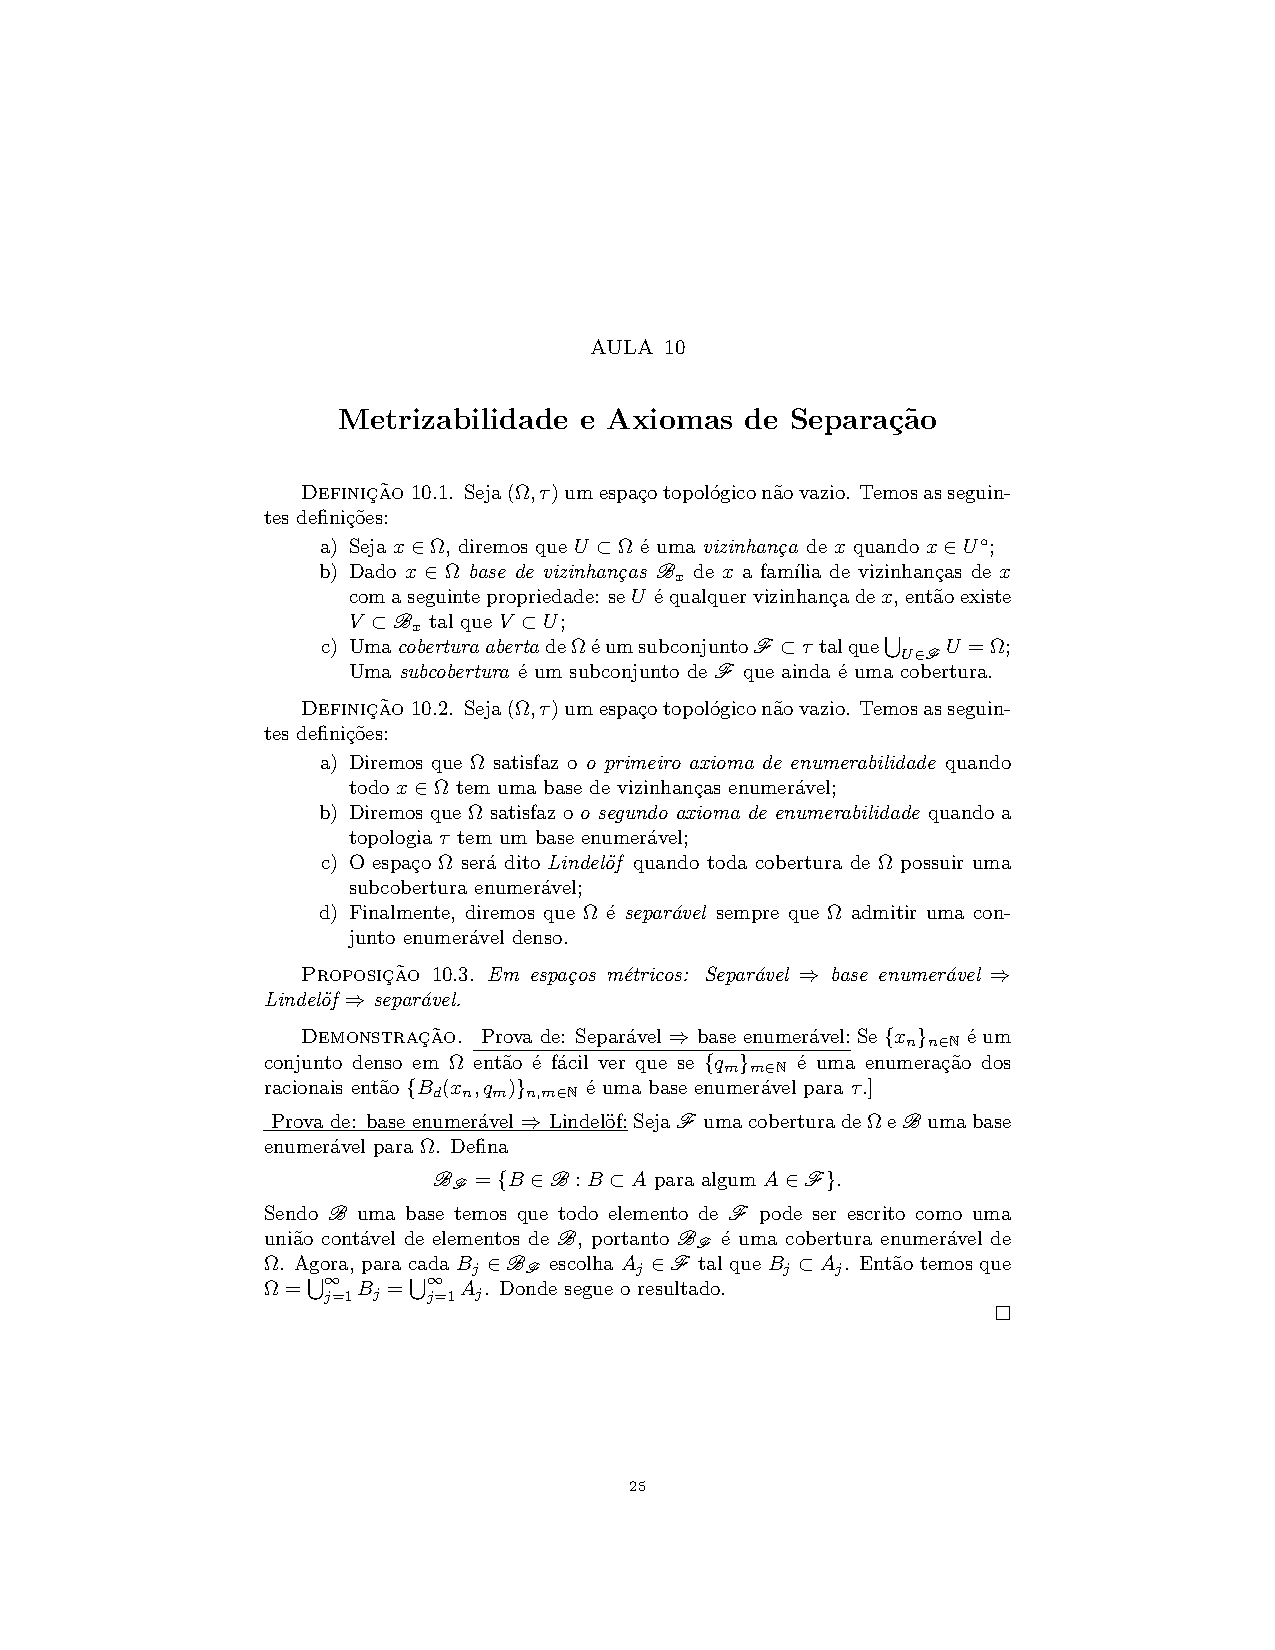
\includepdf[pages=-]{Conexidade_compacidade.pdf}
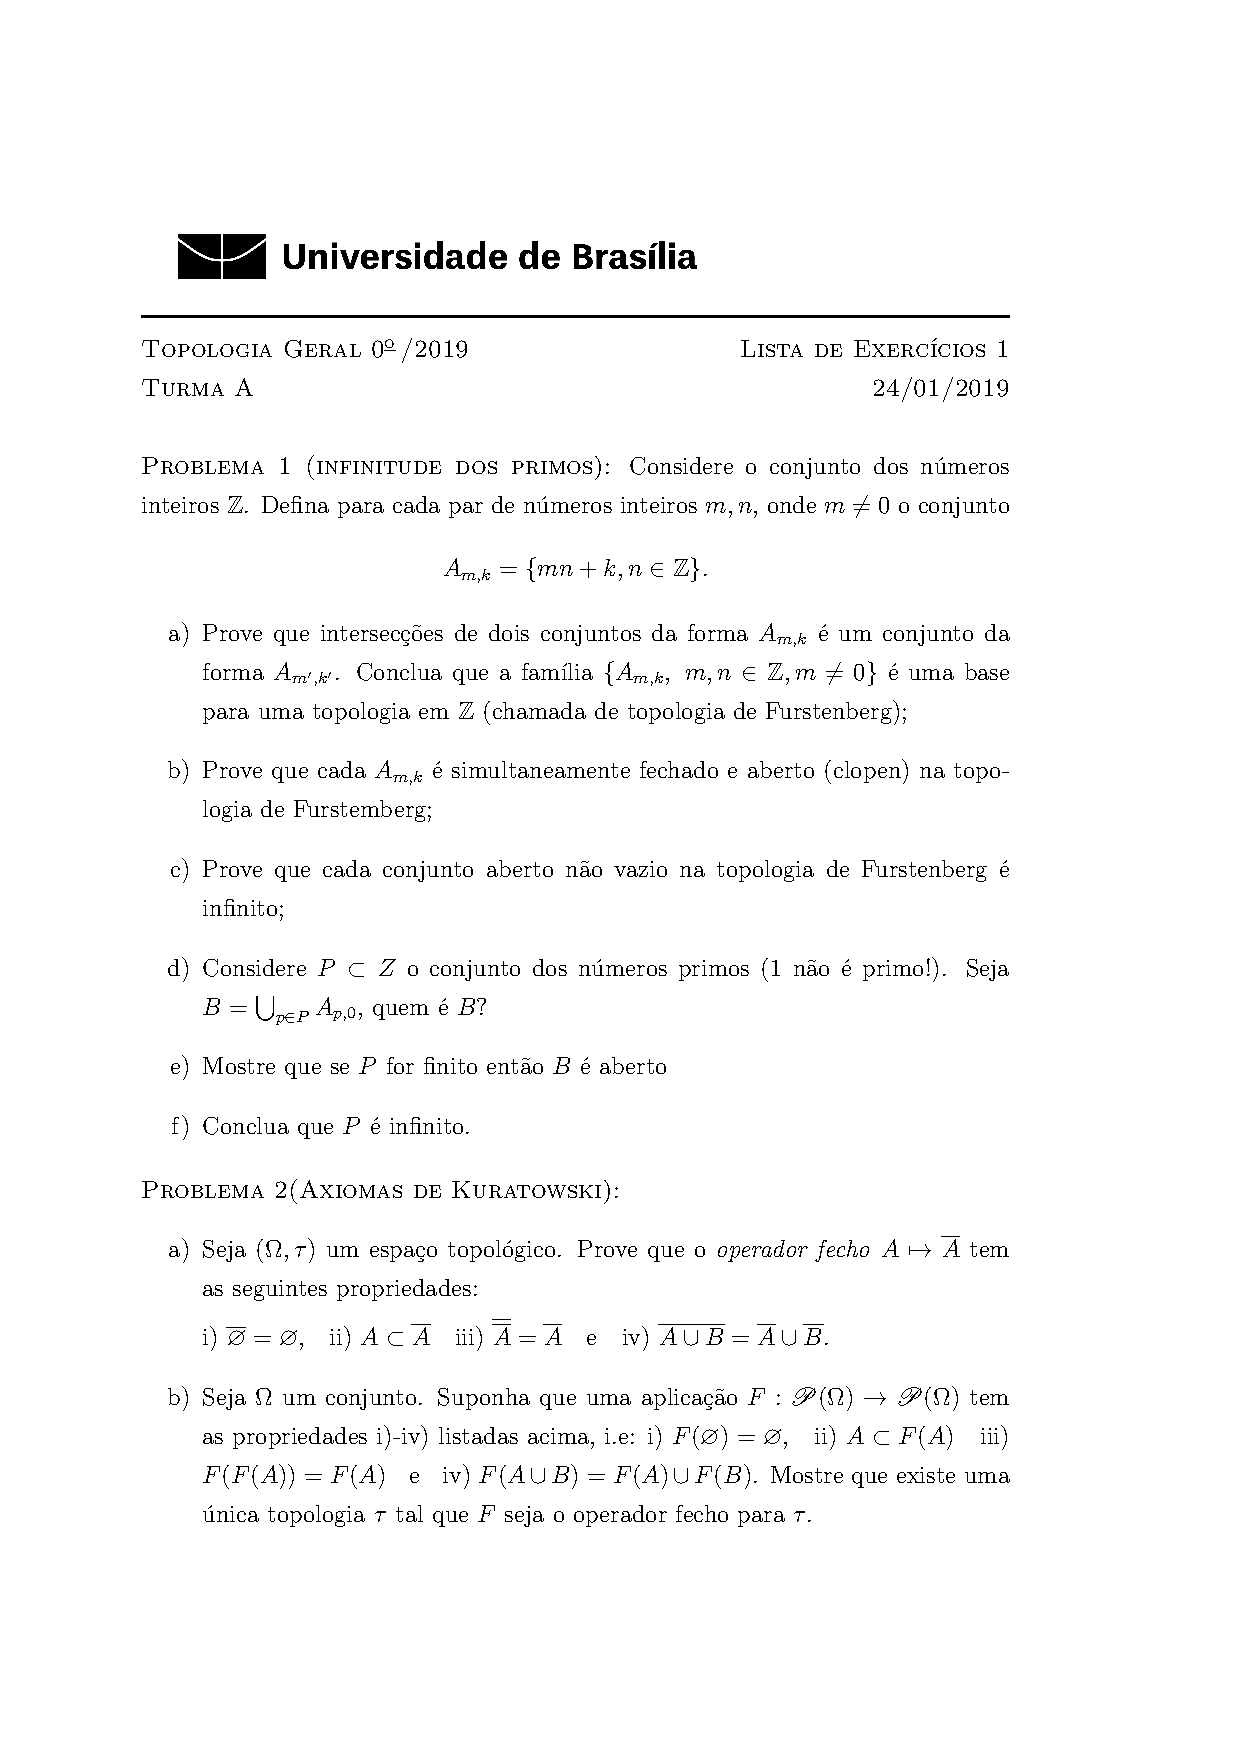
\includepdf[pages=-]{Lista_1.pdf}
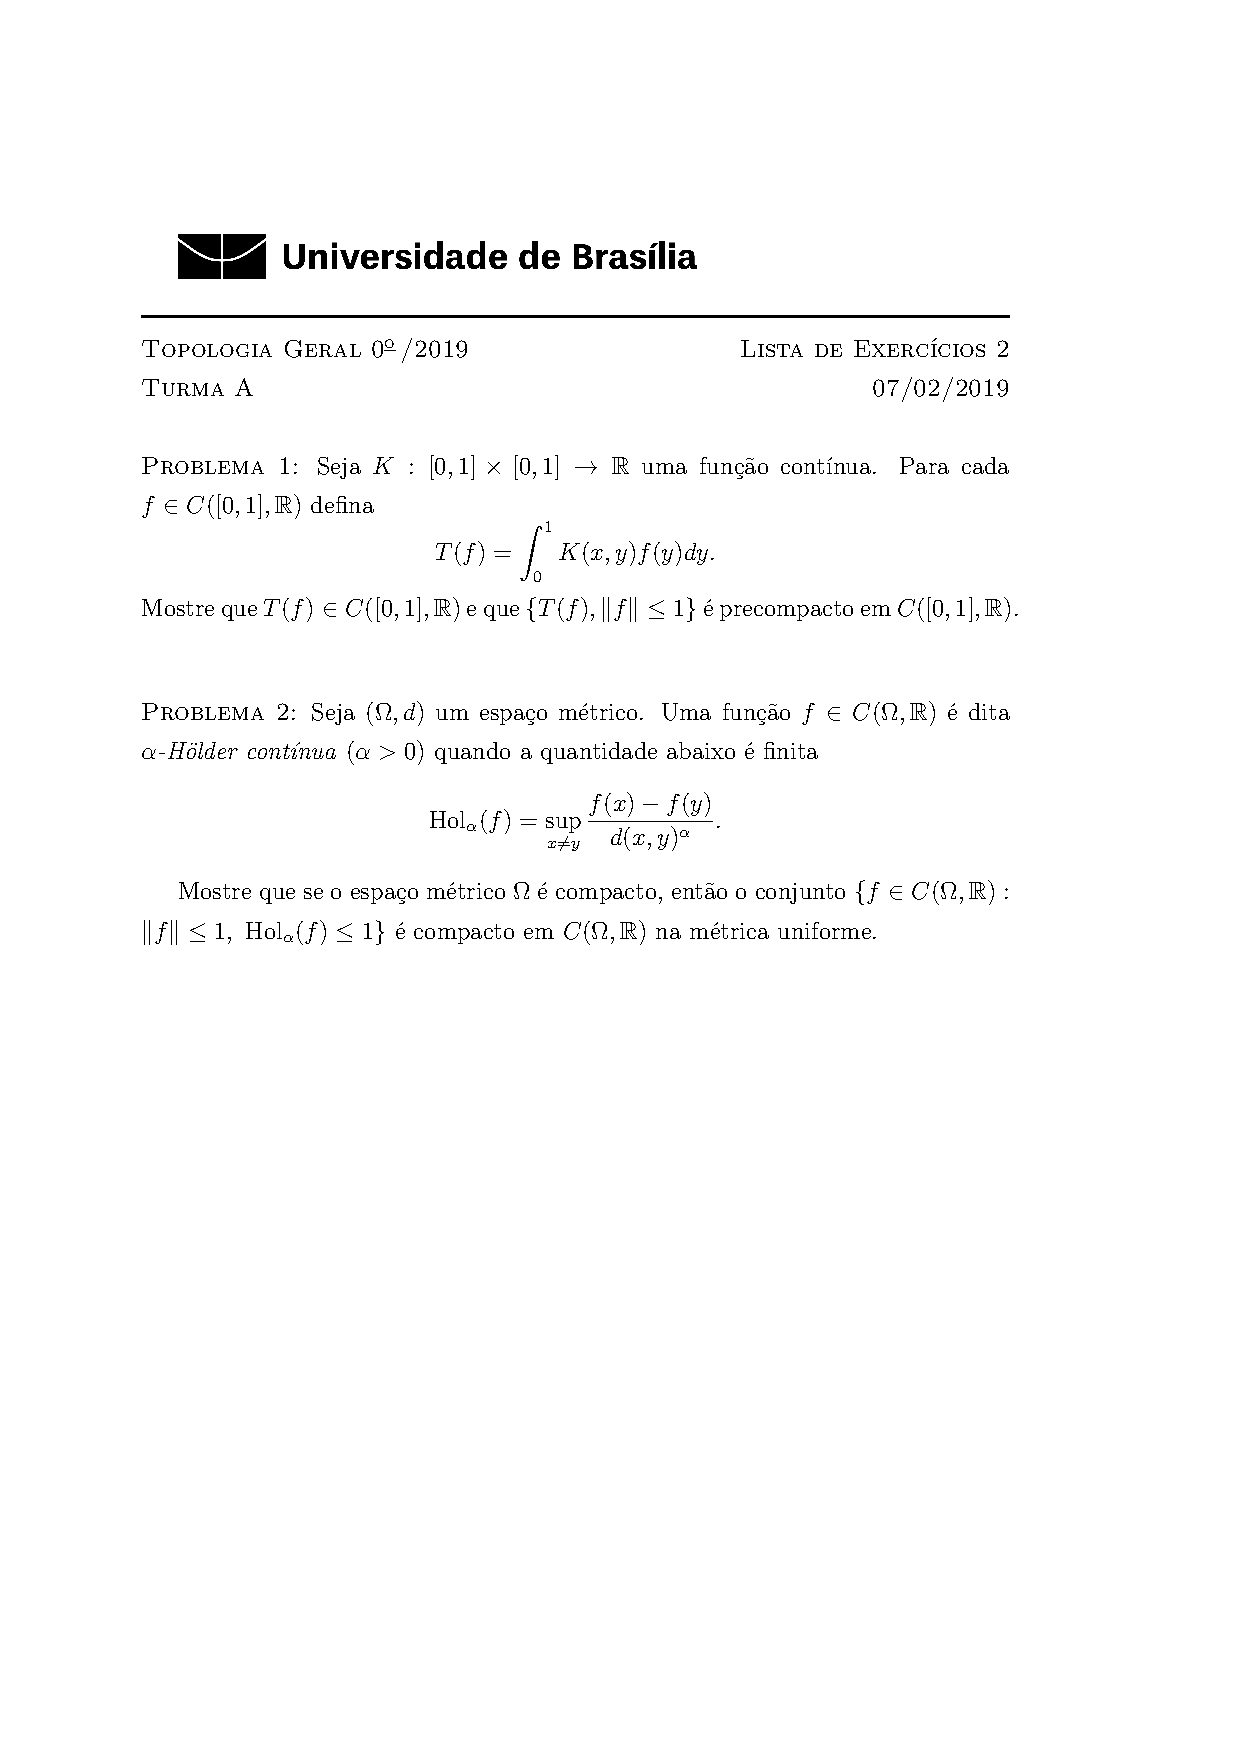
\includepdf[pages=-]{Lista_2.pdf}
\subsection{Resultados auxiliares}
\begin{oobs}
Usaremos implicitamente várias vezes aqui que a união é distributiva sobre a interseção e que a interseção é distributiva sobre a união.
\end{oobs}
\begin{deff}
Uma cisão não trivial de $\Omega$ é um par $U, V$ de abertos não vazios e disjuntos de $\Omega$ cuja união é igual a $\Omega$. Uma cisão trivial de $\Omega$ é um par de abertos disjuntos onde um deles é vazio e o outro é o $\Omega$. $\Omega$ é dito conexo se não existe nenhuma cisão não trivial de $\Omega$ e desconexo caso contrário.
\end{deff}
\begin{deff}
Diremos que $\Omega$ é conexo por caminhos se para todo $x, y \in \Omega$ existe uma função contínua $f: [a,b] \to \Omega$ (que chamaremos de caminho) indo dum fechado da reta em $\Omega$ tal que $f(a) = x$ e $f(b) = y$.
\end{deff}
\begin{deff}
Diremos que $p \in \Omega$ é um ponto de acumulação da sequência $\{x_n \}_{n \in \mathbb{N}} \subset \Omega$ se para toda vizinhança aberta $U$ de $p$ e para todo $n_0 \in \mathbb{N}$ existe $n_1 > n_0$ tal que $x_{n_1} \in U$.
\begin{oobs}
Assumiremos que uma sequência $\{x_n \}_{n \in \mathbf{N}}$ de $\Omega$ é uma função $f: \mathbb{N} \to \Omega$ tal que $f(1) = x_1$ e assim por diante.
\end{oobs}
\begin{oobs}
Com essa definição, um ponto de acumulação de uma sequência $\{x_n \}_{n \in \mathbb{N}}$ não precisa ser um ponto de acumulação de $X = \{x_1, x_2, \cdots \}$ (considere a sequência que alterna entre $0$ e $1$ no compacto $[0,1]$), e a recíproca também não vale (ver a próxima observação).
\end{oobs}

\end{deff}
\begin{oobs}
\textbf{Definição do Munkres}: Diremos que um espaço topológico $\Omega$ é acumuladamente compacto (limit point compact) se todo subconjunto infinito de $\Omega$ tem ponto de acumulação.
\end{oobs}
\begin{oobs}
\textbf{Definição das notas de aula}: Diremos que um espaço topológico $\Omega$ é fracamente sequencialmente compacto se toda sequência $f: \mathbb{N} \to \Omega $ tem ponto de acumulação.
\end{oobs}
\begin{oobs}
A definição do Munkres é mais fraca do que a das notas de aula que exige que toda sequência em $\Omega$ tenha ponto de acumulação: considere a sequência em $\mathbb{N} \times \{0,1 \}$ (onde o primeiro tem a topologia discreta e o segundo a indiscreta) dada por $x_1 = (1, 0), x_2 = (1, 1), x_3 = (2, 0), x_4 = (2, 1), \cdots$, que não tem ponto de acumulação, mas todo $S \subset \Omega$ não vazio (em particular se $S$ é infinito) tem ponto de acumulação (a prova disso é o mesmo argumento usado no exercício $3$ das caixas de compacidade). Porém note que as duas definições são equivalentes se $\Omega$ satisfaz o primeiro axioma de enumerabilidade (ou até mesmo se satisfaz pelo menos que subconjuntos finitos sejam fechados).
\end{oobs}
\begin{oobs}
Ser fracamente sequencialmente compacto é equivalente a ser enumeravalmente compacto (i.e, toda cobertura aberta enumerável tem uma subcobertura aberta finita) e também implica em ser acumuladamente compacto (mas a recíproca só vale se o espaço satisfizer pelo menos que subconjuntos finitos sejam fechados).
\end{oobs}
\begin{lema}\label{sublema}
\textit{Se $C \cup D = \Omega$ é uma cisão não trivial de $\Omega$ e $Y$ é um subespaço conexo de $\Omega$, então ou $Y \subset C$ ou $Y \subset D$. }
\end{lema}
\begin{demm}
Note que $C \cap Y$ e $D \cap Y$ são abertos disjuntos de $Y$ cuja união é todo $Y$, então pela hipótese de conexidade de $Y$ um deles é vazio e outro é todo o $Y$.
\end{demm}
\begin{lema}
\textit{Qualquer conjunto conexo por caminhos é conexo.}
\end{lema}
\begin{demm}
Suponha por absurdo que $\Omega$ é conexo por caminhos mas não é conexo. De fato, se $\Omega = A \cup B$ é uma cisão de $\Omega$, então se $f: [a, b] \to \Omega$ é um caminho arbitrário, como $f([a,b])$ é a imagem contínua de um conexo, também é conexo, e usando o lema \cref{sublema}, temos que $f([a,b])$ ou está contido em $A$ ou em $B$, de forma que não existe nenhum caminho de um ponto de $A$ até um ponto de $B$, uma contradição.
\end{demm}
\begin{lema}\label{lemaDelta}
\textit{Seja $\mathscr{A}$ uma cobertura aberta do espaço métrico $(\Omega, d)$. Se $\Omega$ é sequencialmente compacto, existe $\delta > 0$ tal que todo subconjunto de $\Omega$ com diâmetro menor que $\delta$ está contido em algum elemento de $\mathscr{A}$.}
\end{lema}
\begin{demm}
Suponha por absurdo que $\Omega$ seja sequencialmente compacto mas não existe $\delta$ nas condições do lema. Então, em particular, para cada $n \in \mathbb{N}$, existe um conjunto  $C_n$ de diâmetro menor que $\frac{1}{n}$ que não está contido em nenhum elemento de $\mathscr{A}$. Para cada $n$, escolha um ponto $x_n \in C_n$. Por hipótese, alguma subsequência $\{x_{n_i} \}_{i \in \mathbb{N}}$ da sequência $\{x_n\}_{n \in \mathbb{N}}$ converge para algum ponto $a$. Como $\mathscr{A}$ é cobertura, existe $A \in \mathscr{A}$ tal que $a \in A$. Como $A$ é aberto, existe $\varepsilon > 0$ tal que $B_d(a, \epsilon) \subset A$. Tomando $i$ grande o suficiente de forma que $\mathrm{diam}(C_{n_i}) = \frac{1}{n_i} < \frac{\varepsilon}{2}$  e $d(x_{n_i}, a) < \frac{\varepsilon}{2}$, temos (pela desigualdade triangular) que $C_{n_i} \subset B_d(x_{n_i}, \frac{\varepsilon}{2}) \subset B_d(a, \varepsilon) \subset A$, uma contradição.
\end{demm}
\begin{lema}\label{LemaTres}
\textit{Seja $(\Omega, d)$ um espaço métrico sequencialmente compacto. Então, $\ \forall \varepsilon > 0$, existe uma cobertura finita que consiste de bolas abertas de raio $\varepsilon$.}
\end{lema}
\begin{demm}
Iremos provar a contrapositiva da afirmação, isto é, se existe $\varepsilon > 0$ tal que $\Omega$ não admite nenhuma cobertura finita de bolas abertas de raio $\varepsilon$, então $\Omega$ não é sequencialmente compacto. De fato, se existe tal $\varepsilon$, podemos construir uma sequência $\{x_n\}_{n \in \mathbb{N}}$ que não possui nenhuma subsequência convergente da seguinte maneira: tome $x_1 \in \Omega$ arbitrário e escolha $x_2$ de forma que $x_2 \notin B_d(x_1, \varepsilon)$ (por hipótese podemos fazer isso, senão $B_d(x_1, \varepsilon)$ seria uma cobertura finita de $\Omega$). Em geral, dados $x_1, \cdots, x_n$, tome $x_{n+1} \in \Omega$ de forma que:
$$x_{n+1} \notin B_d(x_1, \varepsilon) \cup B_d(x_2, \varepsilon) \cup \cdots \cup B_d(x_n, \varepsilon)$$
(e novamente, a hipótese garante que possamos fazer isso). É óbvio que, por construção, $d(x_{n+1}, x_i) \geq \varepsilon$ para todo $i \in \{1, \cdots, n \}$, e de fato nenhuma subsequência dessa sequência pode convergir: dado qualquer $x_n$, $B_d(x_n, \frac{\varepsilon}{2})$ contém no máximo um termo da sequência, o próprio $x_n$.
\end{demm}
\begin{lema}
\textit{Seja $(\Omega, d)$ um espaço métrico e $S \subset \Omega$. Então $x \in \Omega$ é ponto de acumulação de $S$ se, e só se, para todo $\varepsilon > 0$, $S \setminus \{x\} \cap B(x, \varepsilon) \neq \emptyset$, isto é, para todo $\varepsilon > 0$, existe $y \neq x \in S$ tal que $d(x, y) < \varepsilon$.}\par
\end{lema}
\begin{demm}
A ida segue diretamente da definição de ponto de acumulação (pois $B(x, \epsilon)$ é um aberto de $\Omega$ contendo $x$) e a volta diretamente do fato de que dado $x \in \Omega$ qualquer aberto $U \ni x$ da topologia gerada por $d$ contém alguma bola de raio $\epsilon$, e portanto $U \cap S \setminus \{ x \} \neq \emptyset$. 
\par
\begin{oobs}
É fácil ver que esse lema também é equivalente a: $x$ é ponto de acumulação de $S \iff$ toda vizinhança aberta de $x$ intersecta $S$ em infinitos pontos distintos.
\end{oobs}
\end{demm}
\begin{lema}\label{LemaCinco}
\textit{Qualquer espaço métrico compacto $(\Omega, d)$ é separável.}
\end{lema}
\begin{demm}
Sabemos que todo espaço métrico compacto $(\Omega, d)$ é totalmente limitado, de forma que para todo $n \in \mathbb{N}$ a cobertura $C_n = \left\{B_d\left(x, \frac{1}{n} \right) \ \vert \ x \in \Omega \right\}$ admite uma subcobertura finita $$F_n = \left\{B_d\left(x_1, \frac{1}{n} \right), B_d\left(x_2,\frac{1}{n} \right), B_d\left(x_3, \frac{1}{n} \right), \cdots, B_d\left(x_k, \frac{1}{n} \right) \right\}$$
para alguns $x_1, \cdots, x_k \in \Omega$. Para cada $n \in \mathbb{N}$, seja $A_n = \{x_1, x_2, \cdots, x_k \}$ o conjunto consistindo dos centros das bolas de $F_n$.  Afirmamos que: $$D = \displaystyle{\bigcup_{n \in \mathbb{N}} A_n}$$
é um subconjunto enumerável de $\Omega$. De fato, $\Omega$ é enumerável, pois é uma união enumerável de conjuntos finitos, e também é denso, pois dado qualquer aberto $U$ não vazio de $\Omega$ e qualquer $x \in U$, então existe $\varepsilon > 0$ tal que $B_d(x, \varepsilon) \subset U$, e tomando $m \in \mathbb{N}$ tal que $\frac{1}{m} < \varepsilon$, então $B_d\left(x, \frac{1}{m} \right) \subset B_d(x, \varepsilon)$. Como $F_m$ é uma subcobertura finita de $\Omega$, existe $y \in A_m$ tal que $x \in B_d\left(y, \frac{1}{m}\right )$, logo $y \in  B_d\left(x, \frac{1}{m}\right )$. Assim:
$$y \in B_d\left(x, \frac{1}{m} \right) \bigcap B_d(x, \varepsilon) \subset D \cap U \neq \emptyset$$
i.e, qualquer aberto não vazio de $\Omega$ intersecta $D$, como desejado.
\end{demm}
\begin{lema}
\textit{Se $(\Omega, d)$ é um espaço métrico, então $d: \Omega \times \Omega \to \mathbb{R}$ é contínua.}
\end{lema}
\begin{demm}
Mostraremos que a imagem inversa de todo aberto $U$ da reta é aberta em $\Omega \times \Omega$. De fato, se $U \subset \mathbb{R}$ é aberto, queremos mostrar que $d^{-1}(U)= \mathscr{O}$ é aberto, isto é, para todo $\mathfrak{o} \in \mathscr{O} $, existe um aberto básico $B$ de $\Omega \times \Omega$ tal que $\mathfrak{o} \in  B \subset \mathscr{O} $. Com efeito, note que se $(x, y) \in d^{-1}(U)$, então $d(x, y) = c \in U$, logo existe $\varepsilon > 0$ tal que $(c - \epsilon, c + \epsilon) \subset U$. Afirmamos que $B = B_d\left(x, \frac{\varepsilon}{2} \right) \times B_d\left(y, \frac{\varepsilon}{2} \right)$ satisfaz o desejado. É óbvio que $(x, y) \in B$, resta mostar que $B\subset \mathscr{O}$. De fato, se $(x', y') \in B$, então note que:
\begin{align}
    |d(x', y') - d(x, y)| &= |d(x', y') - d(x', y) + d(x', y) - d(x, y)|\\
    &\leq |d(x', y') - d(x', y)| + |d(x', y) - d(x, y)| \label{t}\\
    &\leq d(y, y') + d(x, x')\label{y} \\
    &< \dfrac{\varepsilon}{2} + \dfrac{\varepsilon}{2}\\
    &=\varepsilon
\end{align}
logo $d(x', y') \in (c - \varepsilon, c + \varepsilon) \subset U$ e segue que $(x', y') \in \mathscr{O}$. Como $(x, y)$ e $(x', y')$ foram tomados arbitrariamente, o resultado segue.
\end{demm}
\begin{oobs} Para ir de \textcolor{blue}{\textbf{(\ref{t})}} para \textcolor{blue}{\textbf{(\ref{y})}}  note que novamente pela desigualdade triangular:
\begin{align*}
    &d(x', y) - d(y, y') \leq d(x', y') \leq d(x', y) + d(y, y')\\
    &d(x, y) - d(x, x') \leq d(x', y) \leq d(x, x') + d(x, y)
\end{align*}
\end{oobs}
\begin{lema}
\textit{Se $\{A_\alpha \}_{\alpha \in I}$ é uma coleção de subespaços conexos de $\Omega$ e $A$ é um subespaço conexo de $\Omega$ tal que $A \cap A_\alpha \neq \emptyset$ para todo $\alpha \in I$ , então $A \cup \left(\displaystyle{\bigcup_{\alpha \in I} A_\alpha} \right)$ é conexo.}
\end{lema}
\begin{demm}
Note que $A \cup A_\alpha$ é conexo pela proposição \cref{prop126}. Então, novamente pela proposição \cref{prop126}, $\displaystyle{\bigcup_{\alpha \in I}\left(A \cup  \left(\displaystyle{\bigcup_{\alpha \in I} A_\alpha} \right) \right)} = A \cup \left(\displaystyle{\bigcup_{\alpha \in I} A_\alpha} \right)$ é conexo. Note que também poderíamos ter usado o lema \cref{sublema} para mostrar que a única cisão é a trivial.
\end{demm}
\begin{lema}
\textit{Se $A$ e $B$ são subconjuntos próprios de $X$ e $Y$, respectivamente, então $C = X \times Y \setminus A \times B$ é conexo.}
\end{lema}
\begin{demm}
Fixe um $(a_1, a_2) \in C$ de forma que $a_1 \notin A$ e $a_2 \notin B$. Para cada $x \notin A$ defina $V_x = \{x\} \times Y$ e para cada $y \notin B$ defina $H_y = X \times \{y \}$. É claro que ambos são conexos pois são homeomorfos a $X$ e $Y$, respectivamente. Defina $I = \{(x, y) \in X \times Y \ \vert \ x \notin A \text{ e }y\notin B \}$, $D = V_{a_1} \cup H_{a_2}$ e para cada $\alpha \in I$ defina também $A_\alpha = V_{\pi_1(\alpha)} \cup H_{\pi_2(\alpha)}$. Note que:
\begin{enumerate}[label=\color{blue}{\textbf{(\roman*)}}]
    \item $D \cap A_\alpha =\{ (\pi_1(\alpha), a_2), (a_1, \pi_2(\alpha)) \} \neq \emptyset \ \forall \alpha \in I$
    \item $D$ é obviamente a união de subespaços conexos e não disjuntos, donde segue da proposição \cref{prop126} que $D$ é conexo. Analogamente, $A_\alpha$ é também conexo para cada $\alpha \in I$.
\end{enumerate}
e o resultado segue do lema anterior.
\end{demm}
\section{Exercícios de conexidade}
\begin{Mybox}
Prove que a imagem contínua de um espaço conexo é um espaço conexo.
\vspace{-.4cm}
\end{Mybox}
\vspace{-.5cm}
\begin{dem}
Seja $f: X \to Y$ contínua e suponha que $X$ é conexo. Sem perda de generalidade, podemos supor que $f$ é sobrejetiva (caso não fosse, bastaria restringir o contradomínio ao espaço da imagem $Z = f(X)$, que preserva continuidade). Assim, suponha por absurdo que $Z = f(X) = Y =  A \cup B$, i.e, é desconexo. Então, se tomarmos $x \in X$, ou $f(x) \in A$ ou $f(x) \in B$, de onde concluímos que $f^{-1}(A)$ e $f^{-1}(B)$ são abertos (pela hipótese de continuidade) disjuntos cuja união $f^{-1}(A) \cup f^{-1}(B) = X$, ou seja, $X$ é desconexo, um absurdo. 
\end{dem}

\begin{Mybox}
Mostre que:
\begin{enumerate}[label=\color{blue}\normalfont\textbf{(\alph*)}]
\item se $S$ é conexo, então $\overline{S}$ também o é.
\item se $S$ é conexo e $S \subset D \subset \overline{S}$, então $D$ é conexo.
\end{enumerate}
\vspace{-.4cm}
\end{Mybox}
\vspace{-.5cm}
\begin{dem}
\begin{enumerate}[label=\color{blue}\normalfont\textbf{(\alph*)}]
\item Suponha que $S$ seja conexo. Vamos mostrar que a única cisão de $\overline{S}$ é a trivial, isto é, se $\overline{S} = A \cup B$ e $A \neq \emptyset$, então $B = \emptyset$. De fato, temos $A \cap \overline{B} =  \overline{A} \cap B = \emptyset$, e tomando $a \in A$, como $a \notin \overline{B}$, existe $U \ni a$ aberto tal que $U \cap B = \emptyset$, e como $a \in \overline{S}$, existe $x \in U \cap S \neq \emptyset$ com $x \notin B$, assim $x \in S  \cap A \neq \emptyset$. Note que $S = (A \cap S) \cup (B \cap S)$, e pela hipótese de conexidade $B \cap S = \emptyset \implies B = \emptyset$.
\item Suponha por absurdo que $D = A \cup B$ com $A, B$ abertos disjuntos e não vazios. Pelo lema \cref{sublema}, podemos assumir sem perda de generalidade que $S \subset A$, assim $\overline{S} \subset \overline{A}$. Como $\overline{A}$ e $B$ são disjuntos, concluímos que $B = \emptyset$, uma contradição, logo $D$ é conexo.
\end{enumerate}
\end{dem}


\begin{Mybox}
Mostre que:
\begin{enumerate}[label=\color{blue}\normalfont\textbf{(\alph*)}]
\item com a topologia usual, $\mathbb{R}$ é conexo.
\item com a topologia usual, $\mathbb{R}^n$ é conexo.
\end{enumerate}
\vspace{-.4cm}
\end{Mybox}
\vspace{-.5cm}
\begin{dem}
Primeiramente, provaremos a seguinte:
\begin{proposicao}\label{prop126}
Seja $\parent{\Omega, \tau}$ um espaço topológico. Suponha que 
\[
\Omega = \bigcup_{\alpha \in I} S_{\alpha},
\]
onde cada $S_{\alpha}$ é conexo e $\bigcap_{\alpha \in I} S_{\alpha} \neq \emptyset$. Então $\Omega$ é conexo.
\end{proposicao}
\begin{demm}
Suponha que $\Omega = A \cup B$, onde $A$ e $B$ são abertos disjuntos de $\Omega$. Note que para cada $\alpha \in I$, temos que $S_{\alpha} \subset A$ ou $S_{\alpha} \subset B$, pois caso contrário $S_{\alpha}$ não seria conexo. Seja agora $x \in \bigcap_{\alpha \in I} S_{\alpha}$. Se $x \in A$, segue da observação que acabamos de fazer que $S_{\alpha} \subset A$ seja qual for $\alpha \in I$, donde segue que $B = \emptyset$. \emph{Mutatis mutandis}, vemos que se $x \in B$ então $A = \emptyset$. Portanto $\Omega$ é conexo.
\end{demm}
\begin{enumerate}[label=\color{blue}\normalfont\textbf{(\alph*)}]
        \item Temos $\mathbb{R} = \displaystyle{ \bigcup_{n \in \mathbb{N}} [-n, n]}$, uma união de subespaços da reta conexos e não disjuntos. O resultado segue da proposição \cref{prop126}.
        \item Tome $v = (x_1, \cdots, x_n) \in \mathbb{R}^n$ com $||v|| = 1$ e seja $L_v$ a reta de $\mathbb{R}^n$ passando pela origem e com vetor direcional $v$. É claro que $\mathbb{R}^n = \displaystyle{\bigcup_{||v|| = 1} L_v}$, uma união de subespaços de $\mathbb{R}^n$ não disjuntos e conexos (pois são a imagem de $\mathbb{R}$ sob a função contínua $f: \mathbb{R} \to \mathbb{R}^n$ dada por $f(t) = tv$), e o resultado segue da proposição \cref{prop126}.
\end{enumerate}
\end{dem}


\begin{Mybox}
Seja $\parent{\Omega, \tau}$ um espaço topológico. Suponha que cada par de pontos $x, y \in \Omega$ pertença a um conjunto conexo $S_{xy} \subset \Omega$. Então $\Omega$ é conexo.
\vspace{-.4cm}
\end{Mybox}
\vspace{-.5cm}
\begin{dem}
 Fixe algum $x \in \Omega$. Então é claro que $\Omega = \displaystyle{\bigcup_{x \neq y \in \Omega} S_{xy}}$, e o resultado segue da proposição \cref{prop126}.
\end{dem}

\begin{Mybox}
Sejam $\parent{\Omega_1, \tau_1}$ e $\parent{\Omega_2, \tau_2}$ espaços topológicos não vazios. Fixe arbitrariamente $x \in \Omega_1$ e $y \in \Omega_2$. Mostre que $\{x\} \times \Omega_2$ é homeomorfo a $\Omega_2$ e que $\Omega_1 \times \{y \}$ é homeomorfo a $\Omega_1$.
\vspace{-.4cm}
\end{Mybox}
\vspace{-.5cm}
\begin{dem}
É claro que $f: \Omega_2 \to \{x\} \times \Omega_2$ definida por $f(t) = (x, t) \in \{x\} \times \Omega_2$ e $g: \Omega_1 \to \Omega_1 \times \{y\}$ definida por $g(t) = (t, y) \in \Omega_1 \times \{y\}$ são bijeções contínuas com inversas contínuas, como desejado.
\end{dem}

\begin{Mybox}
Mostre que $\mathbb{R}^{\mathbb{N}}$ com a topologia das caixas não é conexo. Sugestão: decomponha $\mathbb{R}^{\mathbb{N}}$ no conjunto das sequências limitadas e das sequências não limitadas.
\vspace{-.4cm}
\end{Mybox}
\vspace{-.5cm}
\begin{dem}
Sejam $A = \{x = (x_1, x_2, \cdots) \in \mathbb{R}^{\mathbb{N}} \ \vert \ \exists K \in \mathbb{R} \text{ tal que } x_n \leq K \ \forall n \in \mathbb{N} \text{ ou } x_n \geq K \ \forall n \in \mathbb{N}\}$ e $B = \{x = (x_1, x_2, \cdots) \in \mathbb{R}^{\mathbb{N}} \ \vert \ \forall M \in \mathbb{R} \ \exists n_M \in \mathbb{N} \text{ tal que } x_{n_M} > M \text{ ou } \forall M \in \mathbb{R} \ \exists n_M \in \mathbb{N} \text{ tal que } x_{n_M} < M\}$. É claro que $A$ e $B$ são subconjuntos de $\mathbb{R}^{\mathbb{N}}$ não vazios cuja união é o próprio $\mathbb{R}^{\mathbb{N}}$. De fato também são abertos, pois dado $x = (x_1, x_2, \cdots) \in \mathbb{R}^{\mathbb{N}}$, ou $x \in A$ ou $x \in B$, e sendo $U$ um aberto básico de $\mathbb{R}^{\mathbb{N}}$ na topologia das caixas dado por:
    $$U = (x_1 - 1, x_1 + 1) \times (x_2 - 1, x_2 + 1) \times \cdots$$
    temos ou $x \in U \subset A$ ou $x \in U \subset B$.
\end{dem}

\begin{Mybox}
Um espaço topológico $\Omega$ é dito ser \emph{totalmente desconexo} quando os únicos subconjuntos conexos de $\Omega$ são os conjuntos unitários. Mostre que se $\Omega$ está equipado com a topologia discreta então $\Omega$ é totalmente desconexo. A recíproca vale?
\vspace{-.4cm}
\end{Mybox}
\vspace{-.5cm}
\begin{dem}
Considerando a topologia discreta, qualquer $V \subset \Omega$ com mais de dois elementos é desconexo, pois fixado $x \in V$, $\{x\} \cup V \setminus \{x \} = V$ é uma união de abertos disjuntos cuja união é $V$. A recíproca não vale, um contra-exemplo é o exemplo $4$ no parágrafo $23$ do Munkres: os racionais com a topologia induzida da reta também são totalmente desconexos.
\end{dem}



\begin{Mybox}
Seja $\colch{A_n}_{n \in \mathbb{N}}$ uma sequência de subespaços conexos de um espaço topológico $\Omega$ que satisfaz $A_n \cap A_{n+1}\neq \emptyset$ seja qual for $n \in \mathbb{N}$. Mostre que $\bigcup_{n \in \mathbb{N}} A_n$ é conexo.  
\vspace{-.4cm}
\end{Mybox}
\vspace{-.5cm}
\begin{dem}
Primeiro provaremos que $\displaystyle{\bigcup_{i = 1}^{n} A_i}$ é conexo para todo $n \in \mathbb{N}$. De fato, pela proposição \cref{prop126}, temos que $A_1 \cup A_2$ é conexo, assim $A_1 \cup A_2 \cup A_3$ também é conexo, também pela proposição \cref{prop126}. Repetindo esse processo, temos que a união finita é conexa. Agora, afirmamos que $$B = \displaystyle{\bigcup_{n \in \mathbb{N}} B_n}$$ é conexo, onde $B_n = \displaystyle{\bigcup_{i = 1}^{n} A_i}$. De fato, usando o lema $23.2$ do Munkres e supondo que haja uma cisão $B = U \cup V$, mostraremos que ou $U = \emptyset$ ou $V = \emptyset$, isto é, $B$ é conexo. Com efeito, como $B_1 \in B$ é conexo e $B_1 \subset B_n \ \forall n \in \mathbb{N}$, então ou $B_1 \subset U $ e $B_n \subset U \ \forall n \in \mathbb{N} \implies U = B \text{ e } V = \emptyset $ ou $B_1 \subset V $ e $B_n \subset V \ \forall n \in \mathbb{N} \implies V = B \text{ e } U = \emptyset$.
\end{dem}


\begin{Mybox}
O espaço topológico $\mathbb{R}_{\ell}$ (\textit{id est,} $\mathbb{R}$ com a topologia do limite inferior) é conexo?
\vspace{-.4cm}
\end{Mybox}
\vspace{-.5cm}
\begin{dem}
 $\mathbb{R}_{\ell}$ não é conexo, pois $\mathbb{R} = (-\infty, 0) \cup [0, \infty)$, uma união de abertos disjuntos na topologia do limite inferior que dá o $\mathbb{R}$ todo.
\end{dem}


\begin{Mybox}
Mostre que um espaço topológico $\Omega$ é conexo se, e somente se, as únicas funções $f: \Omega \to \{0, 1 \}$ contínuas são as constantes.
\vspace{-.4cm}
\end{Mybox}
\vspace{-.5cm}
\begin{dem}
Primeiro provaremos a contrapositiva de $\text{conexo} \implies  \text{únicas funcões contínuas são constantes}$. De fato, se $f: \Omega \to \{0, 1\}$ é não constante e contínua, então, como $\{0, 1 \}$ é clopen independente de sua topologia, por hipótese $f^{-1}(\{0, 1\})$ é um clopen não vazio de $\Omega$, i.e, $\Omega$ é desconexo. Reciprocamente, se $\Omega = A \cup B$ com $A$ e $B$ abertos não vazios disjuntos, note que $f: \Omega \to \{0, 1\}$ definida pondo $f(x) = 0$ se $x \in A$ e $f(x) = 1$ se $x \in B$ é não constante e contínua. 
\end{dem}

\begin{Mybox}
Mostre que para cada $n \geq 2$, $\mathbb{R}^n \setminus \{x_1, \ldots, x_n \}$ é conexo.
\vspace{-.4cm}
\end{Mybox}
\vspace{-.5cm}
\begin{dem}
\textbf{Sem usar conexidade por caminhos:} Tome:
        \begin{align*}
         &A = \{(\pi_1(x_1), \cdots, \pi_{n-1}(x_1)) , (\pi_1(x_2), \cdots, \pi_{n-1}(x_2)), \cdots (\pi_1(x_k), \cdots, \pi_{n-1}(x_k)) \}\\
        &B = \{\pi_n(x_1), \cdots, \pi_n(x_k) \}
        \end{align*}
        e note que $$(\mathbb{R}^{n-1} \times \mathbb{R}) \setminus (A \times B) \subset \mathbb{R}^{n} \setminus \{x_1, \cdots, x_k \} \subset \underbrace{\overline{(\mathbb{R}^{n-1} \times \mathbb{R}) \setminus (A \times B)}}_\text{$= \mathbb{R}^n$, pois $A \times B$ é finito}$$
        portanto o resultado segue do lema $8$ e da $b)$ do segundo exercício das caixas de conexidade. \par 
\textbf{Usando conexidade por caminhos:} Iremos mostrar a condição mais forte de que $\mathbb{R}^n \setminus F$, onde $F \subset \mathbb{R}^n$ é finito, é conexo por caminhos (e é fácil ver que todo espaço conexo por caminhos é conexo). De fato, dado $x,y \in \mathbb{R}^n$, há uma quantidade infinita (\textit{e não enumerável}) de retas passando por $x$ que não intersectam $F$, escolha aleatoriamente alguma dessas retas e seja $\alpha$ a sua inclinação. É claro que também há uma quantidade infinita (\textit{e não enumerável}) de retas passando por $y$ com inclinação $\beta \in \mathbb{R} \setminus \{\alpha\}$ que não intersectam $F$, escolha também uma dessas retas e seja $\beta$ a sua inclinação. Como $L_\alpha$ e $L_\beta$ tem inclinações diferentes, sua interseção é não vazia. Basta então tomar algum $p$ nessa interseção e notar que o caminho que vai de $x$ a $p$ contido em $L_\alpha$ e depois de $p$ a $y$ contido em $L_\beta$ é contínuo. Note que poderíamos enfraquecer a condição de $F$ ser finito, a prova também funciona se $F$ for só enumerável.
\end{dem}

\begin{Mybox}
Mostre que $\mathbb{R}^2 \setminus \mathbb{Q}^2$ é conexo. 
\vspace{-.4cm}
\end{Mybox}
\vspace{-.5cm}
\begin{dem}
Observe que $\mathbb{Q}^2$ é enumerável. A prova é idêntica à do exercício anterior (uma prova mais fácil é notar que dado dois pontos $p, q$ com coordenadas irracionais, eles podem ser conectados pelo caminho que passa pelo ponto intermediário $(\sqrt{2}, \sqrt{2})$ por segmentos de retas horizontais e verticais).
\end{dem}

\begin{Mybox}
Mostre que $\mathbb{R}^n$ e $\mathbb{R}$ não são homeomorfos para todo $n \geq 2$.
\vspace{-.4cm}
\end{Mybox}
\vspace{-.5cm}
\begin{dem}
 $\mathbb{R} \setminus \{0\}$ é desconexo, mas para $n \geq 2$ tirar qualquer ponto de $\mathbb{R}^n$ ainda o deixa conexo. Como conexidade é um invariante topológico (ou seja, se dois espaços são homeomorfos ou ambos são conexos ou ambos são desconexos), o resultado segue.
\end{dem}

\begin{Mybox}
Seja $E \subset \mathbb{R}^n$ um subespaço de codimensão $\geq 2$. Mostre que $\mathbb{R}^n \setminus E$ é conexo.
\vspace{-.4cm}
\end{Mybox}
\vspace{-.5cm}
\begin{dem} \\
\textbf{Sem usar conexidade por caminhos:} Suponha que $\codim(E) \geq 2$, ou, equivalentemente que $\dim(E) = j \leq n - 2$. Faça uma mudança de base* de forma que:
    $$v \in E \iff v = \left(\displaystyle{\sum_{i = 1}^{j} \phi_i e_i} \right) + 0e_{j+1} + \cdots + 0e_n$$
    para alguns $\phi_i, \cdots, \phi_j \in \mathbb{R}$, onde $\{e_1, \cdots, e_j  \}$ é uma base de $E$ e $\{e_{j+1}, \cdots, e_n \}$ é uma base do seu complemento ortogonal. Defina a família $\{A_{\alpha_1, \cdots, \alpha_j} \}_{\alpha_1, \cdots, \alpha_j \in \mathbb{R}}$ da seguinte maneira:
    $$\textit{Fixados $\alpha_1, \cdots, \alpha_j \in \mathbb{R}$, então } v \in A_{\alpha_1, \cdots, \alpha_j} \iff v = \left(\displaystyle{\sum_{i=1}^{j} \alpha_i e_i}\right) + \beta_1 e_{j+1} + \cdots + \beta_{n-j} e_{n}  $$
    onde exigiremos que $\beta_i \neq 0$ para pelo menos algum $i \in \{1, \cdots, n-j \}$. É claro que $A_{\alpha_1, \cdots, \alpha_j} \cong \mathbb{R}^{n-j}\setminus \{\mathbf{0} \}$, que é conexo (\textit{note que justamente aqui que usamos a hipótese da codimensão ser pelo menos $2$!}). Agora, fixe $\mathbf{0} \neq a = (a_{j+1}, \cdots, a_n) \in \mathbb{R}^{n-j}$ e defina outro subespaço $A$ homeomorfo ao $\mathbb{R}^j$ da seguinte maneira:
    $$v \in A \iff v = \left(\displaystyle{\sum_{i = 1}^{j}\gamma_i e_i} \right) + a_{j+1} e_{j+1} + \cdots a_n e_n$$
    (note que aqui não exigimos nada dos $\gamma$). É claro que $A \cong \mathbb{R}^j$ e que* $A \cap A_{\alpha_1, \cdots, \alpha_j} \neq \emptyset$ para todos $\alpha_1, \cdots, \alpha_j \in \mathbb{R}$. Note também que*:
    $$A \cup \left(\displaystyle{\bigcup_{\alpha_1, \cdots, \alpha_j \in \mathbb{R}} A_{\alpha_1, \cdots, \alpha_j}} \right) = \mathbb{R}^n \setminus E$$
    e o resultado segue do lema $7$.
    \begin{oobs}
    \textit{Isso sempre é possível pois $E \cong \mathbb{R}^j$.}
    \end{oobs}
    \begin{oobs}
    \textit{Note que se $(\alpha_1, \cdots, \alpha_j) \neq \mathbf{0}$ então $(\alpha_1, \cdots, \alpha_j, a_{j+1}, \cdots, a_n)$ é testemunha desse fato.}
    \end{oobs}
    \begin{oobs}
    \textit{A primeira inclusão é provada da seguinte maneira: se $v \in A$ ou $v \in \displaystyle{\bigcup_{\alpha_1, \cdots, \alpha_j \in \mathbb{R}} A_{\alpha_1, \cdots, \alpha_j}} $, então suas $j$-ésimas primeiras coordenadas são combinações lineares de vetores da base de $E$ mas há pelo menos uma coordenada das $n-j$ restantes que não é nula, de forma que $v \in \mathbb{R}^n \setminus E$. Reciprocamente, se $v \in \mathbb{R}^n \setminus E$, então ou todas as coordenadas a partir da $j+1$-ésima são iguais às de $a$ ou isso não acontece. No primeiro caso temos $v \in A$ e no segundo temos $v \in \displaystyle{\bigcup_{\alpha_1, \cdots, \alpha_j \in \mathbb{R}} A_{\alpha_1, \cdots, \alpha_j}}$.}
    \end{oobs}
\textbf{Usando conexidade por caminhos:} Seja $F$ um subespaço complementar de $E$, isto é, $\mathbb{R}^n =  E \oplus F$. Tome $x, y \in \mathbb{R}^n \setminus E$ e denote por $\Bar{x}, \Bar{y}$ as suas projeções em $F$. Afirmamos que o seguinte caminho liga $x$ a $y$: $$x \to \Bar{x} \to_{*} \Bar{y} \to y$$ onde cada $\to$ denota um segmento de reta, e devemos tomar o cuidado de não passar pela origem indo de $\Bar{x}$ a $\Bar{y}$ (o que é facilmente realizado: escolha retas passando por $\Bar{x}$ e por $\Bar{y}$ que não passam pela origem se intersectam em $p$ e tome o caminho $\Bar{x} \to p \to \Bar{y}$).
\begin{oobs}
A recíproca desse exercício também vale (e é mais fácil de provar), i.e, se $E$ é um subespaço vetorial, $\mathbb{R}^n \setminus E$ ser conexo implica que $\dim(E) \leq n -2$.
\end{oobs}
\end{dem}
\section{Exercícios de compacidade}
\begin{Mybox}
Seja $K \subset \Omega$. Então $K$ é compacto se, e somente se, toda cobertura de $K$ por abertos de $\Omega$ admite uma subcobertura finita.
\vspace{-.4cm}
\end{Mybox}
\vspace{-.5cm}
\begin{dem}
Suponha que $K$ é compacto e $\mathscr{A} = \{A_{\alpha}\}_{\alpha \in J}$ é uma cobertura de $Y$ por abertos de $\Omega$. Então é claro que: $$\{A_{\alpha} \cap K \ \vert \ \alpha \in J \ \}$$ é uma cobertura de $K$ por abertos de $K$, e por hipótese uma subcobertura finita da forma: $$\{A_{\alpha_1} \cap K, \cdots, A_{\alpha_n} \cap K \}$$ cobre $K$. Segue que $\{A_{\alpha_1}, \cdots, A_{\alpha_n} \}$ é uma subcobertura de $\mathscr{A}$ que cobre $K$. 
    \par 
    Reciprocamente, se toda cobertura de $K$ por abertos de $\Omega$ tem uma subcobertura finita que cobre $K$, mostraremos que $K$ é compacto. De fato, se $\mathscr{A}' = \{A_{\alpha}' \}$ é uma cobertura de $K$ por abertos de $K$, então, por definição de topologia induzida, temos que para cada $A'_{\alpha}$, existe $A_\alpha$ aberto de $\Omega$ tal que: $$A'_{\alpha} = A_\alpha \cap K$$ Temos que $\mathscr{A} = \{A_\alpha \}$ é uma cobertura de $K$ por abertos de $\Omega$, então por hipótese existe alguma subcobertura finita $\{A_{\alpha_1}, \cdots, A_{\alpha_n} \}$ que cobre $K$, segue que $\{A'_{\alpha_1}, \cdots, A'_{\alpha_n} \}$ é uma subcobertura finita de $\mathscr{A}'$ que cobre $K$.
\end{dem}


\begin{Mybox}
Mostre que um espaço métrico é fracamente sequencialmente compacto se, e somente, se, é sequencialmente compacto. Se $\Omega$ for apens um espaço topológico, qual dessas noções implica a outra? Dê um exemplo de um espaço não metrizável em que essas noções não coincidem.
\vspace{-.4cm}
\end{Mybox}
\vspace{-.5cm}
\begin{dem}
Se toda sequência em um espaço métrico tem ponto de acumulação, então é claro que toda sequência tem uma subsequência convergente, basta usar a definição para bolas abertas de raios cada vez menores com centros todos no ponto de acumulação, identicamente ao que é feito abaixo. Para a recíproca basta usar o teorema $13.11$ e a proposição $13.8$ das notas de aula. Um contra-exemplo que satisfaz o pedido no final do exercício é o seguinte:\par
    Tome $I = [0,1]$ e considere $I^I$ com a topologia produto. Temos que o mesmo é compacto pelo teorema de Tychonoff e portanto fracamente sequencialmente compacto, mas a sequência de funções $\alpha_n \in I^I$ definida por: $$\alpha_n(x) \doteq \text{ o enésimo dígito na expansão binária de $x$}$$ não tem subsequência convergente. De fato, suponha por absurdo que $\{\alpha_{n_k} \}_{k \in \mathbb{N}}$ é uma subsequência que converge a algum $\alpha \in I^I$, então para cada $x \in I$,  $\alpha_{n_k}(x)$ converge a $\alpha(x) \in I$. Defina $p \in I$ com a propriedade de que $\alpha_{n_k}(p) = 0 \text{ ou }1$ dependendo da paridade de $k$. Então a sequência $\{\alpha_{n_k} \}_{k \in \mathbb{N}}$ é dada por $0, 1, 0, 1, \cdots$, que obviamente não pode convergir.
    
    \textit{\textbf{Prova de que em espaços métricos ser acumuladamente compacto é equivalente a ser sequencialmente compacto, mas que em espaços topológicos em geral a recíproca não vale: }}\textit{Suponha que $(\Omega, d)$ seja fracamente sequencialmente compacto, i.e, todo subconjunto infinito tem um ponto de acumulação. Dado uma sequência $\{x_n \}_{n \in \mathbb{N}}$, se a mesma só tiver uma quantidade finita de termos distintos, então trivialmente contém uma subsequência constante e portanto convergente. Caso a sequência contenha infinitos termos distintos, por hipótese tem um ponto de acumulação $x$, então defina a seguinte subsequência $\{x_{n_i} \}_{i \in \mathbb{N}}$, escolhendo $x_{n_1}, x_{n_2}, \cdots$ de forma que:}
    $$x_{n_1} \in B_d(x, 1)$$ 
    \textit{e defina $n_i$ indutivamente, em termos de $n_{i-1}$, tal que $n_i > n_{i-1}$ e:}
    $$x_{n_{i}} \in B_d\left(x, \frac{1}{i}\right)$$
    \textit{o que sempre podemos fazer, já que $B_d\left(x, \frac{1}{i}\right)$ intersecta $A$ em infinitos pontos distintos*. Então é claro que $x_{n_i} \rightarrow x$. Como $\{x_n \}_{n \in \mathbb{N}}$ foi escolhida arbitrariamente, segue que $\Omega$ é sequencialmente compacto.} \par
    \textit{Reciprocamente, vamos provar que se $\Omega$ é sequencialmente compacto, então é compacto (e sabemos que isso implicará que $\Omega$ é fracamente sequencialmente compacto, como desejado). Por hipótese valem o lema $2$ e $3$, portanto existe uma cobertura finita de bolas abertas de raio $\varepsilon = \frac{\delta}{3}$ (onde $\delta$ é como no lema \cref{lemaDelta}) e diâmetro $\frac{2\delta}{3}$, de forma que cada uma está contida em algum $A \in \mathscr{A}$. O conjunto consistindo de todos os $A$ dessa forma é obviamente uma subcobertura finita de $\Omega$, como desejado.}\par
    \textit{Um exemplo de um espaço acumuladamente compacto mas não sequencialmente compacto (e portanto não metrizável) é $\mathbb{R}$ com a topologia gerada por $\{(a, \infty) \ \vert \ a \in \mathbb{R} \}$. Qualquer subconjunto $A \subset \mathbb{R}$ não vazio tem pontos de acumulação, pois dado $a \in A$, $a - \epsilon$ é ponto de acumulação de $A$, já que $(a- \epsilon, \infty) \cap A \setminus \{a - \epsilon \} = a$. Note que a sequência  definida por $x_n = -n$ não tem subsequência convergente nessa topologia.}
\end{dem}

\begin{Mybox}
Seja $\Omega = \{0, 1 \}$ e considere em $\Omega$ a topologia $\tau = \{\emptyset, \Omega \}$. Equipe $\mathbb{N}$ com a topologia discreta e considere o produto $\mathbb{N} \times \Omega$. Use esse exemplo para mostrar que nem todo espaço fracamente sequencialmente compacto é compacto.
\vspace{-.4cm}
\end{Mybox}
\vspace{-.5cm}
\begin{dem}
Afirmamos que nas condições do exercício, qualquer conjunto não vazio de $\mathbb{N} \times \{0, 1\}$ tem pontos de acumulação. De fato, se $S \subset \mathbb{N} \times \{0, 1\}$ é não vazio, então existe $n \in \mathbb{N}$ tal que ou $(n, 0) \in S$ e claramente $(n, 1)$ é ponto de acumulação (qualquer aberto básico da topologia produto contendo $(n, 1)$ intersecta $S$ em $(n, 0) \neq (n,1)$) ou, analogamente, $(n, 1) \in S$ e $(n, 0)$ é ponto de acumulação. Finalmente, note que $\mathscr{U} = \{U_n\}_{n \in \mathbb{N}} = \{\{n \} \times (0,1) \}_{n \in \mathbb{N}}$ é uma cobertura aberta infinita que não admite subcobertura aberta finita.
\end{dem}

\begin{Mybox}
Considere o cubo de Hilbert $C = [0, 1]^{\mathbb{N}}$ equipado com a métrica produto, i.e, $d(x, y) = \sup_{n \in \mathbb{N}} \colch{\frac{|x_n - y_n|}{n}}$.
\begin{enumerate}[label=\color{blue}\normalfont\textbf{(\alph*)}]
\item Mostre que nessa topologia, bolas $B_d(x, r)$ são conjuntos da forma $\prod_{n \in \mathbb{N}} B(x_n, nr)$ (aqui $B$ sem o índice indica a bolas de $[0, 1]$ relativas ao valor absoluto);
\item Mostre que $C$ é completo;
\item Verifique que $C$ é totalmente limitado e conclua que $C$ é compacto. 
\end{enumerate}
\vspace{-.4cm}
\end{Mybox}
\vspace{-.5cm}
\begin{dem}

\begin{enumerate}[label=\color{blue}\normalfont\textbf{(\alph*)}]
\item Note que, dado $r > 0$ e tomando $N \in \mathbb{N}$ tal que $\frac{1}{N} <r $, temos:
        \begin{align}
            &y \in \displaystyle{\prod_{n \in \mathbb{N}} B(x_n, nr)} \iff \dfrac{|x_n - y_n|}{n} < r \ \forall n \in \mathbb{N}\\
            &\iff \displaystyle{\sup_{n \in \mathbb{N}}\left\{\dfrac{|x_n - y_n|}{n} \right\} = \max \left\{|x_1 - y_1|, \dfrac{|x_2 - y_2|}{2}, \cdots, \dfrac{|x_{N-1} - y_{N-1}|}{N-1},\sup_{n \geq N }\left\{\dfrac{|x_n - y_n|}{n} \right\} \right\} } < r \\
            &\iff y \in B_d(x, r)
        \end{align}
        onde na penúltima igualdade que cada um dos termos dentro dos colchetes é menor que $r$ (veja a observação seguinte), e portanto o seu máximo também é menor que $r$. \par
        \begin{oobs}
        \textit{Para $n < N$ isso é trivial, note que se $n \geq N$, temos $\frac{|x_n - y_n|}{n} \leq \frac{1}{n} \leq \frac{1}{N} \implies \displaystyle{\sup_{n \geq N }\left\{\dfrac{|x_n - y_n|}{n} \right\} \leq \frac{1}{N} < r}$}
        \end{oobs}
\item Seja $\{x_k \}_{k \in \mathbb{N}} \subset [0,1]^{\mathbb{N}}$ uma sequência de Cauchy, com $x_k = (x_k^{(1)},x_k^{(2)}, \cdots) \in [0,1]^{\mathbb{N}}$. Queremos mostrar que $\{x_k \}_{k \in \mathbb{N}}$ converge, isto é, achar uma sequência $y = (y^{(1)}, y^{(2)}, \cdots) = (y^{(j)})_{j \in \mathbb{N}}$ tal que $d(x_k, y) \to 0$. Faremos isso da seguinte forma:
        \begin{enumerate}[label=\color{blue}{\textbf{(\roman*)}}]
            \item\label{passoI} Mostraremos que se $\{x_k \}_{k \in \mathbb{N}}$ é de Cauchy, então $\{x_k^{(j)} \}_{k \in \mathbb{N}} = \{\pi_j(x_k) \}_{k \in \mathbb{N}} \subset [0,1]$ converge para cada $j \in \mathbb{N}$.
            \item Usando um exercício de uma lista passada (questão $6$ do parágrafo $19$ do Munkres), concluíremos que $\{x_k \}_{k \in \mathbb{N}}$ converge. A completude de $[0,1]^\mathbb{N}$ segue imediatamente.
        \end{enumerate}
        De fato, dados $\varepsilon > 0$ e $j_0 \in \mathbb{N}$ arbitrários, então, por hipótese, existe $K \in \mathbb{N}$ tal que $k_1, k_2 \geq K$ implica que:
            $$d(x_{k_1}, x_{k_2}) = \displaystyle{\sup_{n \in \mathbb{N}}} \left\{\dfrac{\left|x_{k_1}^{(n)} - x_{k_2}^{(n)} \right|}{n}  \right\} < \dfrac{\varepsilon}{j_0}$$
        Mas também é óbvio que:
        $$\dfrac{\left|x_{k_1}^{(j_0)} - x_{k_2}^{(j_0)}\right|}{j_0} \leq  \displaystyle{\sup_{n \in \mathbb{N}}} \left\{\dfrac{\left|x_{k_1}^{(n)} - x_{k_2}^{(n)} \right|}{n}  \right\} < \dfrac{\varepsilon}{j_0} \implies \left|x_{k_1}^{(j_0)} - x_{k_2}^{(j_0)}\right| < \varepsilon$$
        de onde segue que $\{x_k^{(j)} \}_{k \in \mathbb{N}} $ é de Cauchy e portanto converge a algum $y^{(j)}$ (logo o passo \ref{passoI} foi realizado). Como desejado, concluímos que $\pi_j(x_k) \to \pi_j(y)$ para cada $j \in \mathbb{N}$, onde $y = (y^{(1)}, y^{(2)}, \cdots) = (y^{(j)})_{j \in \mathbb{N}}$.
        \item Seja $\varepsilon > 0$ arbitrário e tome $n \in \mathbb{N}$ tal que $\frac{1}{N} < \frac{\varepsilon}{2}$. Para cada $i > N$, tome $p_i = 1$. Fixe $i \in \{1, \cdots, N \}$. Como $[0,1]$ é totalmente limitado, existe um número finito de pontos $\{x_1, x_2, \cdots, x_M\} = A_0$ tal que:

        $$x \in [0, 1] \implies |x - x_j| < \frac{\varepsilon}{2} \text{ para algum $j \in \{1, \cdots, M\}$}$$ 
        
        Agora, defina $A = \{x = (x_n)_{n \in \mathbb{N}} \in [0,1]^{\mathbb{N}} \ \vert \ x_1, x_2, \cdots, x_N \in A_0 \text{ e } x_{N+1} = x_{N+2} = \cdots = 1  \}$. Existem $M^N$ pontos em $A$, portanto $A$ é finito. Além do mais, se $x = (x_n)_{n \in \mathbb{N}} \in [0,1]^{\mathbb{N}}$, então para cada $i \in \{1, \cdots, N\}$, existem $x^{(i)}_j \in A_0$ (o que significa que todos os $x_j$ dependem dos $i$) tal que $|x_i - x^{(i)}_j | < \frac{\varepsilon}{2}$. Agora, se definirmos $y_i = x^{(i)}_j $ para $i \in \{1, \cdots, N\}$ e $y_i = 1$ caso contrário, então por construção $y = (y_n)_{n \in \mathbb{N}} \in A$, e para cada $i \in \{1, \cdots, N\}$, temos que $\frac{|x_i - y_i|}{n} \leq |x_i - y_i| < \frac{\varepsilon}{2}$, também para cada $i > N$, vale que $\frac{|x_i - y_i|}{i} \leq \frac{1}{i} < \frac{1}{N} < \frac{\varepsilon}{2}$, logo $\displaystyle{\sup_{n \in \mathbb{N}}} \left\{\dfrac{\left|x_n - y_n \right|}{n} \right\} \leq \frac{\varepsilon}{2} < \varepsilon$ e segue que $[0,1]^{\mathbb{N}} = \displaystyle{\bigcup_{a \in A}B(a,\varepsilon)}$.
\end{enumerate}
\end{dem}

\begin{Mybox}
Seja $\Omega$ um espaço compacto Hausdorff. Seja $f: \Omega \cup \{\infty\} \to \mathbb{R}$ uma função semicontínua inferiormente. Então $f$ é limitada inferiormente, i.e, $\inf_{x \in \Omega} f(x) > -\infty$, e existe $x \in \Omega$ tal que $f(x) = \inf_{x \in \Omega} f(x)$. 
\vspace{-.4cm}
\end{Mybox}
\vspace{-.5cm}
\begin{dem}
 \begin{oobs} 
    Há um erro de digitação no enunciado. Apesar de não fazer diferença, a questão é: \textit{Seja $\Omega$ um espaço compacto Hausdorff. Seja $f: \Omega \to \mathbb{R} \cup \{ \infty\}$ semicontínua inferiormente. Então $f$ é limitada inferiormente, i.e, o infímo da imagem de $\Omega_1$ existe e $f$ atinge seu ínfimo em $\Omega_1$.}
    \end{oobs}
    Seja* $m = \inf f(\Omega)$. Para cada $n$, defina $C_n = f^{-1}(\left(-\infty, m + \frac{1}{n} \right])$. Note que $C = \{C_n \}$ satisfaz a propriedade da interseção finita, pois:
\begin{align*}
    &f^{-1}\left(\left(-\infty, m + \frac{1}{n_1}\right]\right) \bigcap f^{-1}\left(\left(-\infty, m + \frac{1}{n_2}\right]\right)\bigcap \cdots \bigcap f^{-1}\left(\left(-\infty, m + \frac{1}{n_k}\right]\right)\\
    &=f^{-1}\left(\left(-\infty, m + \frac{1}{n_1}\right] \bigcap \left(-\infty, m + \frac{1}{n_2}\right] \cdots \bigcap \left(-\infty, m + \frac{1}{n_k}\right] \right)\\
    &=f^{-1}\left(\left(-\infty, m + \frac{1}{n_j}\right] \right) \text{, onde $n_j = \max\{n_1, \cdots, n_k\}$}\\
    &\neq \emptyset \text{ pela definição de infímo}
\end{align*}
Logo (pois $\Omega$ é compacto), $\displaystyle{\bigcap_{n \in \mathbb{N}} C_n} \neq \emptyset$. Mas se $x \in \displaystyle{\bigcap_{n \in \mathbb{N}} C_n}$, então $f(x) \leq m$, e como $m$ é infímo, $f(x) = m$ e segue que $f$ atinge seu ínfimo, como desejado.\par
\begin{oobs}
\textit{O ínfimo de $f(\Omega)$ existe, pois $\{U_\alpha \}_{\alpha \in \mathbb{R}}$, com $U_\alpha = f^{-1} ((\alpha, \infty))$ é uma cobertura aberta que admite subcobertura finita e portanto $f(\Omega)$ é limitado por baixo.}
\end{oobs}
\begin{oobs}
\textit{Note que provamos algo mais forte, pois em momento algum usamos a hipótese de que $\Omega$ é Hausdorff (só de ser compacto já basta). Note também que o $\infty$ foi colocado no exercício sem necessidade. Caso o erro de digitação não fosse erro de digitação, teríamos que o $\infty$ foi introduzido sem propósito algum, jogado fora depois. Se não tivesse sido jogado fora o exercício também estaria falso (pois sequer especifica a topologia de $\Omega \cup \{ \infty\}$), considere $\Omega =[0,1]$ e coloque em $\Omega \cup \{\infty\}$ a topologia $\tau_{[0,1]} \cup \{\{\infty \}, \Omega \cup \{\infty \}  \}$, então pondo $f(x) = 2$ se $x \in [0,1]$ e $f(\infty) = 1$, $\inf f(\Omega \cup \{\infty\})$ não é atingido em $\Omega$.}
\end{oobs}
\end{dem}

\begin{Mybox}
Considere $[0, 1]^{\mathbb{N}}$ com a topologia uniforme. Encontre nesse espaço um subconjunto infinito sem pontos de acumulação.
\vspace{-.4cm}
\end{Mybox}
\vspace{-.5cm}
\begin{dem}
 \begin{oobs}
    \textit{A métrica da topologia uniforme é dada por:
    $$d ( \mathbf { x } , \mathbf { y } ) = \sup \left\{ \overline { d } \left( x _ { \alpha } , y _ { \alpha } \right) | \ \alpha \in J \right\}$$
    onde $\overline{d}$ é a métrica limitada padrão de $\mathbb{R}$.}
    \end{oobs}
    Agora, para cada $j \in \mathbb{N}$ defina $e_j \in [0,1]^{\mathbb{N}}$ pondo $\pi_i(e_j) = 1$ se $i = j$ e $\pi_i(e_j) = 0$ caso contrário. Afirmamos que $E = \displaystyle{\bigcup_{j \in \mathbb{N}} \{e_j \}} = \{e_j \}_{j \in \mathbb{N}}\subset [0,1]^{\mathbb{N}} $ não tem pontos de acumulação. De fato, se $p \in [0,1]^{\mathbb{N}}$ é ponto de acumulação, então $B = B_d\left(p, \frac{1}{3} \right)$ (onde $d$ é a métrica da topologia uniforme), então por hipótese existem infinitos pontos distintos de $E$ em $B$. Isso é um absurdo, pois $B$ não pode conter nem mesmo dois pontos distintos de $E$: se $i \neq k$, então $d(e_i, e_k) = 1 > \displaystyle{\sup_{x, y \in B} d(x, y) } = \diam(B) = \frac{2}{3}$. \par
    
    \textit{Prova alternativa: de fato, lembrando do lema \cref{LemaTres}, se pormos $\varepsilon = \frac{1}{2}$, por exemplo, então dado $e_k \in E$, para todo $e_j \neq e_k$, temos $d(e_k, e_j) = 1 > \frac{1}{2}$, por exemplo, então dado $e_k \in E$, para todo $e_j \neq e_k$, temos $d(e_k, e_j) = 1 > \frac{1}{2}$, e portanto nenhum ponto de $E$ é ponto de acumulação. Mostraremos agora que também vale que nenhum ponto fora de $E$ é ponto de acumulação, e portanto $E'$ é vazio: 
    \\
    Dado $x \in E^c$, podemos supor que existe $j_0 \in \mathbb{N}$ tal que $a = d(x, e_{j_0}) \in (0,1)$  (caso contrário teríamos $d(x, e_n) = 1$ para todo $n \in \mathbb{N}$ e a prova acabaria). Pela desigualdade triangular, para todo $i \neq j$, temos; $$d(x, e_i) + d(x, e_j) = d(e_i, x) + d(x, e_j) \geq d(e_i, e_j) = 1 \implies d(x, e_i ) \geq 1 - d(x,e_j)$$ para todo $j \neq i$. Em particular, $d(x, e_i) \geq 1 - a > \frac{1-a}{2}$ para todo $i \neq j_0$. Assim, temos que $d(x, e_i) > \max\{\frac{1-a}{2}, \frac{a}{2} \}$ para todo $i \in \mathbb{N}$ e segue que $x$ não é ponto de acumulação.}
\end{dem}

\begin{Mybox}
Mostre que $[0, 1]$ como subespaço de $\mathbb{R}_{\ell}$ não é f.s.c.
\vspace{-.4cm}
\end{Mybox}
\vspace{-.5cm}
\begin{dem}
Aqui mostraremos que $[0,1]$ como subespaço de $\mathbb{R}_l$ não é acumuladamente compacto. O resultado seguirá imediatamente, pois se fosse fracamente sequencialmente compacto, seria acumuladamente compacto, como já observado anterioremente. \par 
    Mostraremos que $A = \left\{1 - \dfrac{1}{n} \right\}_{n \in \mathbb{N}}$ não tem pontos de acumulação. De fato, se $x = 1 - \dfrac{1}{n} \in A$, então temos $$1 - 1 / n \in \left[ 1 - \frac { 1 } { n } , 1 - \frac { 1 } { n + 1 } \right)$$ mas $\left[ 1 - \frac { 1 } { n } , 1 - \frac { 1 } { n + 1 } \right) \cap A \setminus \{x\} = \emptyset$, logo $x$ não é ponto de acumulação. Caso $x \in (0,1)$ com $x \notin A$, então $x \in \left[ 1 - \frac { 1 } { j } , 1 - \frac { 1 } { j + 1 } \right) = U _ { x }$ para algum $j \in \mathbb{N}$ mas $\left[x, 1 - \frac{1}{j+1} \right) \cap A = \emptyset $ e então $x$ não é ponto de acumulação. Trivialmente se $x > 1$ ou $x <0$ então $x$ não é ponto de acumulação, então resta mostrar que $1$ não é ponto de acumulação. Isto é claro, pois $[1, 2) \cap [0,1] = \{ 1 \}$.
    \begin{oobs}
    \textit{Uma solução mais direta e elegante é notar que todo ponto de acumulação numa topologia mais fina é necessariamente ponto de acumulação na topologia mais grossa, portanto se $A$ tivesse pontos de acumulação em $\mathbb{R}_l$ eles teriam de ser pontos de acumulação de $A$ em $\mathbb{R}$ também, mas o único ponto de acumulação de $A$ em $\mathbb{R}$ é $1$, que não é ponto de acumulação de $A$ em $\mathbb{R}_l$ pois $\{ 1 \} = [0, 1] \cap [1, 2)$ é um aberto de $[0,1]$ que não intersecta $A$.}
    \end{oobs}
\end{dem}

\begin{Mybox}
Mostre que o círculo $\mathbb{S}^1$ com a topologia induzida de $\mathbb{R}^2$ é compacto. 
\vspace{-.4cm}
\end{Mybox}
\vspace{-.5cm}
\begin{dem}
Mostraremos que $\mathbb{S}^1$ é fechado e limitado, seguirá que é compacto. De fato $\mathbb{S}^1$ é fechado, pois $\mathbb{S}^1 = f^{-1}(\{1\})$, imagem inversa de fechado e portanto fechado, onde $f(x, y) = x^2 + y^2$. É limitado pois está contido na bola aberta (com a topologia padrão de $\mathbb{R}^2$) de centro $(0,0)$ e raio $2$.
\end{dem}



\begin{Mybox}
Mostre que $[0, 1]$ não é compacto como subespaço de $\mathbb{R}_K. $
\vspace{-.4cm}
\end{Mybox}
\vspace{-.5cm}
\begin{dem}
É fácil ver que $\{U_n \}_{n \in \mathbb{N}}$, onde: $$U_n = \left\{\left(\dfrac{1}{n}, 2 \right) \right\}_{n \in \mathbb{N}} \bigcup \ (-1,1) - K$$ é uma cobertura aberta que não admite subcoobertura aberta finita.
\end{dem}

\begin{Mybox}
Seja $\{x_n \}_{n \in \mathbb{N}} \subset \mathbb{R}$ uma sequência convergente com limite $x$. Mostre que $\{ x\} \cup \{x_n \}_{n \in \mathbb{N}}$ é compacto. 
\vspace{-.4cm}
\end{Mybox}
\vspace{-.5cm}
\begin{dem}
Seja $\mathscr{A}$ uma cobertura aberta de $\Omega = \{x \} \cup \{x_n \ \vert \ n \in \mathbb{N} \}$ .Como $\mathscr{A}$ é cobertura, existe $A_0 \in \mathscr{A}$ contendo $x$. Como $A_0$ é uma vizinhança aberta de $x$ e por hipótese $x_n \to x$, $A_0$ contém todos termos da sequência a partir de certo $N \in \mathbb{N}$, isto é, existe $N \in \mathbb{N}$ tal que $\{x_N, x_{N+1}, \cdots \} \in A_0$. Para cada $x_i$ com $1 \leq i \leq N - 1$, usaremos que $\mathscr{A}$ é cobertura e escolheremos $A_1, \cdots, A_{N-1} \in \mathscr{A}$ tal que $x_i \in A_i$ para todo $1 \leq i \leq N - 1$. Então é claro que: $$\{A_0, A_1, \cdots, A_{N-1} \}$$ é uma subcobertura aberta finita de $\Omega$.
\end{dem}

\begin{Mybox}
Mostre que qualquer espaço métrico compacto $\Omega$ é homeomorfo a algum subconjunto do cubo de Hilbert. (Sugestão $\Omega$ é separável (justifique), então seja $\{ x_1, x_2, \ldots\}$ um subconjunto denso em $\Omega$. Defina $F: \Omega \to C$ pondo $F(x) = \parent{d(x, x_1), d(x, x_2), \ldots}$ e mostre que $F$ é um homeomorfismo).
\vspace{-.4cm}
\end{Mybox}
\vspace{-.5cm}
\begin{dem}
Já provamos que $(\Omega,d)$ é separável no lema \cref{LemaCinco} e sabemos que qualquer função contínua e bijetora de um espaço compacto num espaço Hausdorff é um homeomorfismo.  Note que, sem perda de generalidade, podemos assumir que $d(x, y) \leq 1$ para todo $x, y \in \Omega$ (se isso não acontecesse poderíamos simplesmente usar a métrica limitada padrão, que é equivalente). Sendo $A = \{x_1, x_2, \cdots \}$ um subconjunto denso de $\Omega$, então afirmamos que o homemomorfismo desejado é:
    \begin{align*}
        &F: (\Omega, d) \to F(\Omega) \subset C = [0,1]^{\mathbb{N}}\\
        &x \mapsto (d(x, x_1), d(x_, x_2), \cdots)
    \end{align*}
    onde a topologia em $F(\Omega)$ é a induzida de $C$. De fato, como $F$ é por construção sobrejetiva e $F(\Omega)$ é Hausdorff (pois $[0,1]^\mathbb{N}$ é Hausdorff e obviamente qualquer subespaço de um espaço Hausdorff é Hausdorff também), tudo que nos resta é provar que $F$ é injetora (já que - pelo lema $6$ - as funções coordenadas de $F$ são contínuas e portanto $F$ é contínua). Ora, se $f(x) = f(y)$ para $x, y \in \Omega$, então:
    \begin{align*}
        &d(x, x_1) = d(y, x_1) \\
        &d(x, x_2) = d(y, x_2) \\
        &\vdots\\
        &d(x, x_n) = d(y, x_n) \ \forall n \in \mathbb{N}
    \end{align*}
    e note que, como $A$ é denso, então para todo $\varepsilon > 0$, existe $x_k \in A$ tal que $d(x, x_k) = d(y, x_k) < \frac{\varepsilon}{1332}$. Segue que para todo $\varepsilon > 0$, temos: $$d(x, y) \leq d(x, x_k) + d(y, x_k) < \frac{\varepsilon}{1332} + \frac{\varepsilon}{1332} =\frac{ \varepsilon}{666} < \varepsilon$$
    e concluímos que $x = y$. 
\end{dem}
\fakesection{Resolução da lista 1}
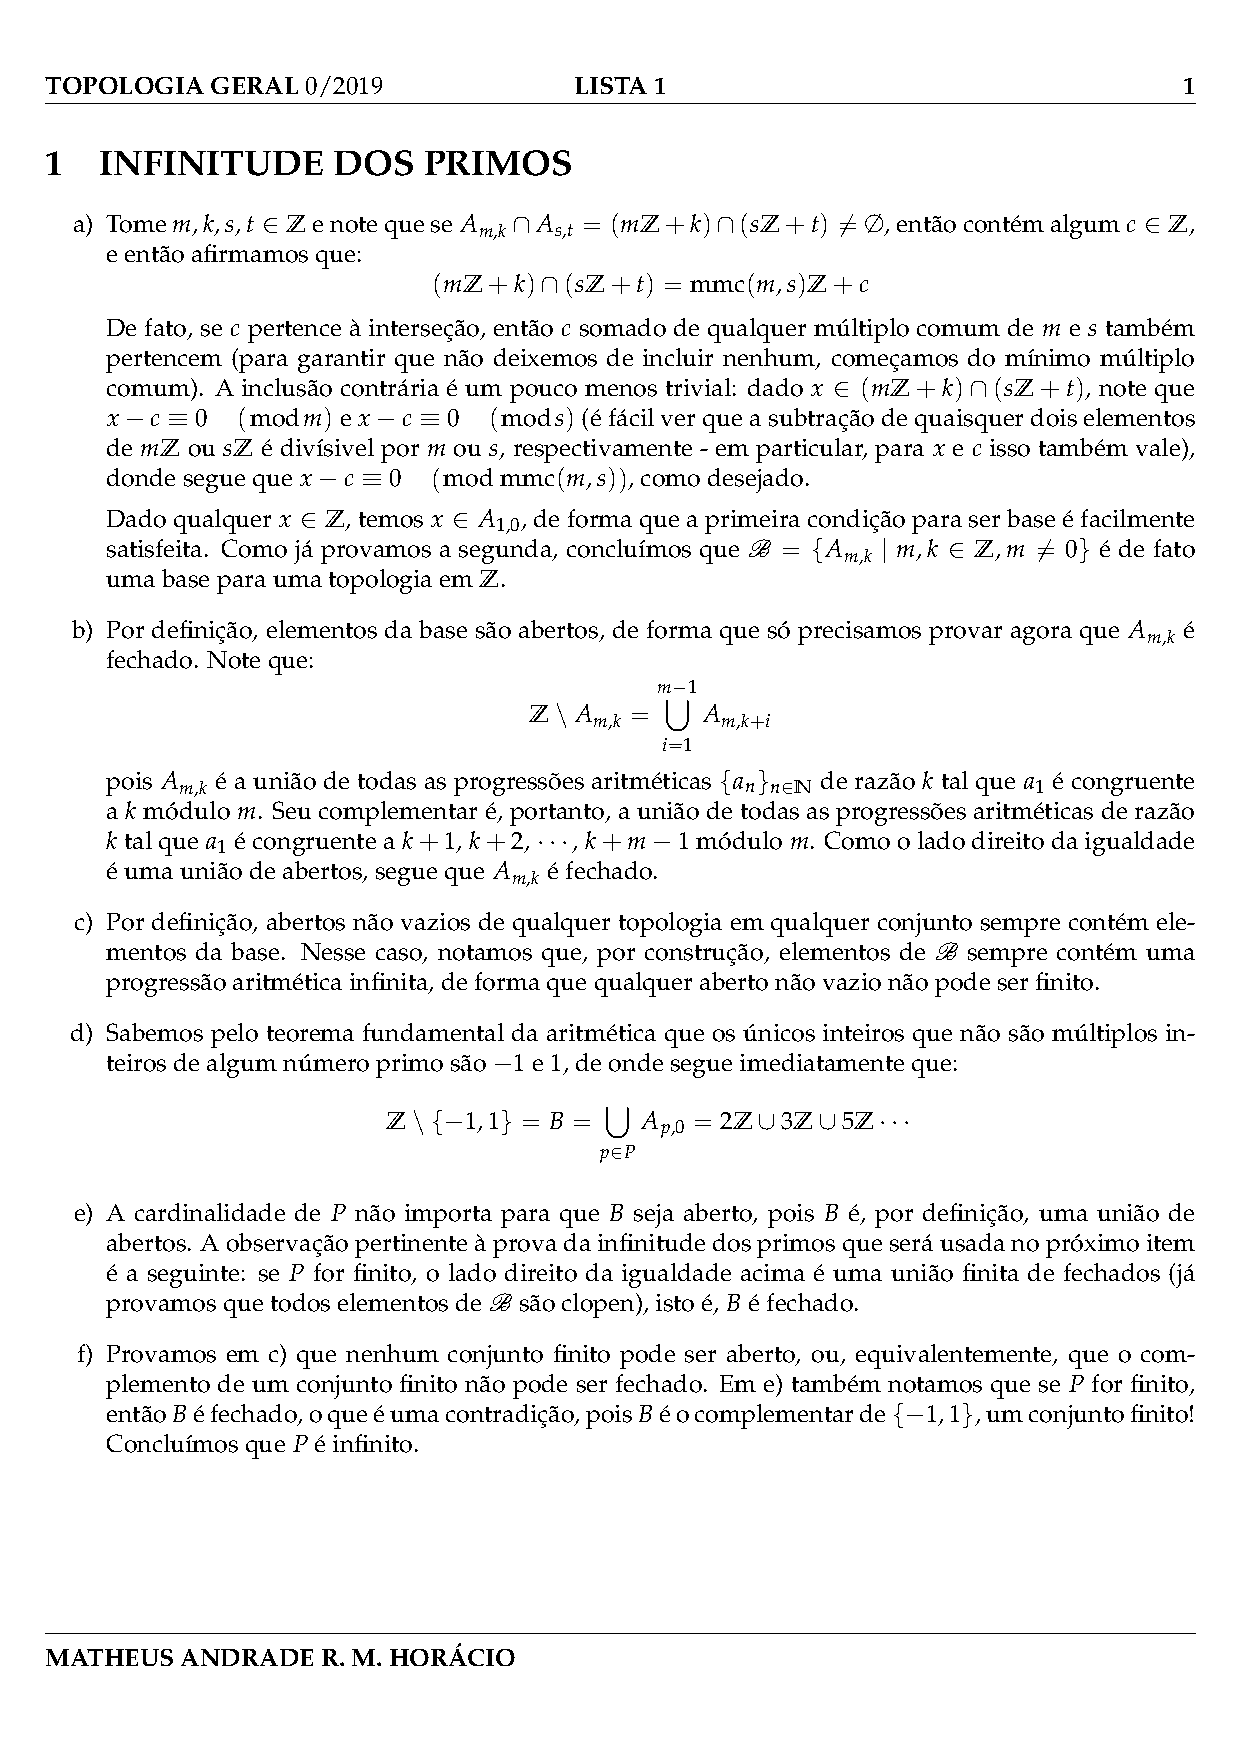
\includepdf[pages=-]{SolLista1.pdf}
\fakesection{Resolução da lista 2}
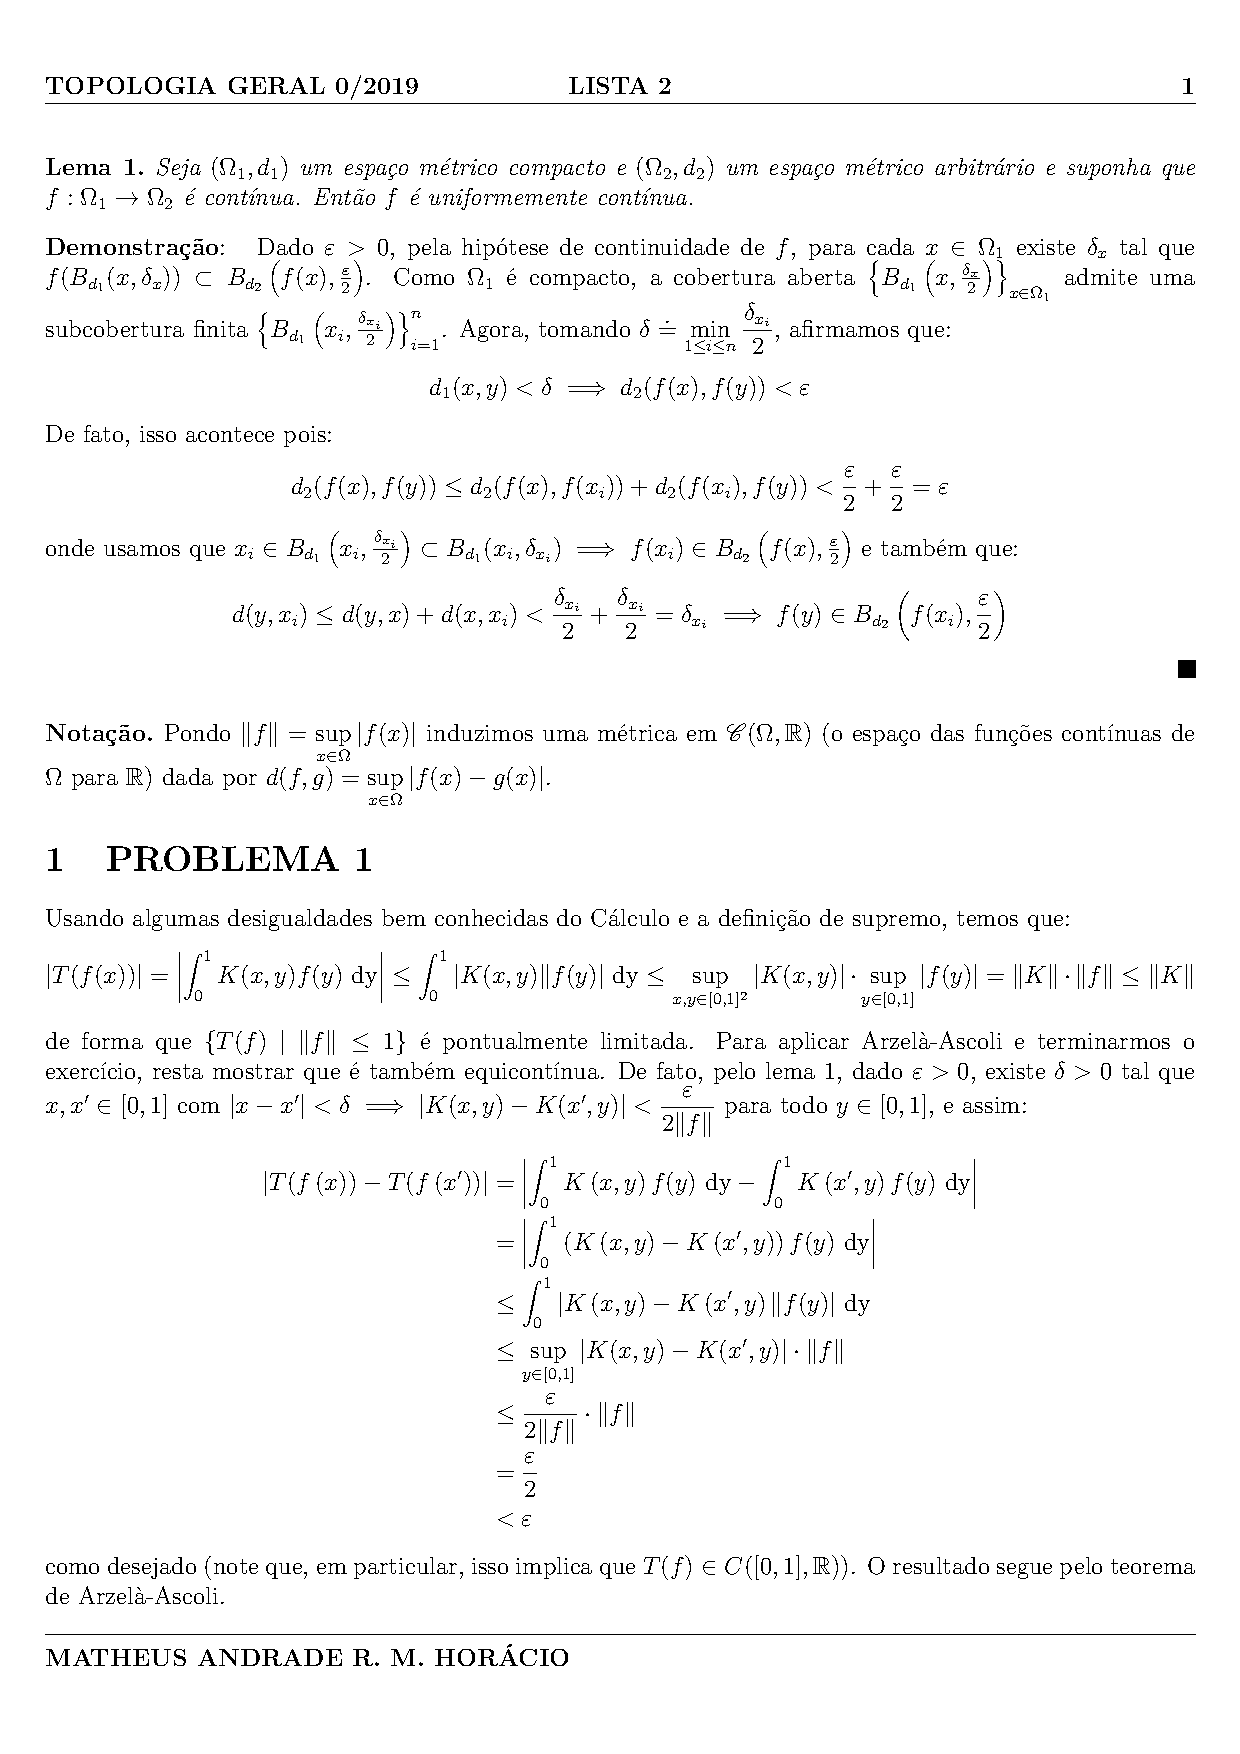
\includepdf[pages=-]{SolLista2.pdf}


\end{document}